%; whizzy paragraph
%; whizzy-paragraph "^\\\\dancersection"
% -initex iniptex -latex platex -format platex -bibtex jbibtex -fmt fmt
% 以上 whizzytex を使用する場合の設定。

%     Tokyo Debian Meeting resources
%     Kansai Debian Meeting resources
%     Copyright (C) 2008 Junichi Uekawa
%     Copyright (C) 2008 Nobuhiro Iwamatsu

%     This program is free software; you can redistribute it and/or modify
%     it under the terms of the GNU General Public License as published by
%     the Free Software Foundation; either version 2 of the License, or
%     (at your option) any later version.

%     This program is distributed in the hope that it will be useful,
%     but WITHOUT ANY WARRANTY; without even the implied warranty of
%     MERCHANTABILITY or FITNESS FOR A PARTICULAR PURPOSE.  See the
%     GNU General Public License for more details.

%     You should have received a copy of the GNU General Public License
%     along with this program; if not, write to the Free Software
%     Foundation, Inc., 51 Franklin St, Fifth Floor, Boston, MA  02110-1301 USA

%   Pdf作成手順
% dvipdfmx debianmeetingresume2011-fuyu.dvi
%  preview (shell-command (concat "evince " (replace-regexp-in-string "tex$" "pdf"(buffer-file-name)) "&"))
% 画像ファイルを処理するためにはebbを利用してboundingboxを作成。
%(shell-command "cd image2012-fuyu; ebb *.png")


% progress memo:
% 2015/6-2015/11がマージ対象
% イベント等でない場合は理由を書くこと。
% 必要な変更点は FIXME で記録しています。

%%ここからヘッダ開始。

\documentclass[mingoth,a4paper]{jsarticle}
\usepackage{monthlyreport}
\usepackage[dvips]{xy} % for advi workaround. Bug #452044
\usepackage{iwamatsu}
\usepackage{ulem}

% ページ調整のため部分的に2段組に
\usepackage{multicol}

\begin{document}

\begin{titlepage}
\thispagestyle{empty}

\hspace*{-2.5cm}
\includegraphics{image2012-natsu/gudeb.eps}\\
\\
\\
\rotatebox{10}{\fontsize{32}{32} {\gt 東京エリア/関西Debian勉強会}}

%\vspace*{-1.5cm}
\hspace*{11cm}
\includegraphics[height=6cm]{image200502/openlogo-nd.eps}\\
\vspace*{0.1cm}
\hfill あんどきゅめんてっど でびあん 2015年冬号 2015年12月31日 初版発行
\end{titlepage}

\newpage
\thispagestyle{empty}\mbox{}
\newpage

% section の代わりの環境 -- 改訂する。
\renewcommand{\dancersection}[2]{%
\newpage
あんどきゅめんてっど でびあん 2015年冬号
%
% top line
\vspace{0.1mm}\\
{\color{dancerlightblue}\rule{\hsize}{2mm}}

%
% middle text
%
\begin{minipage}[t]{0.6\hsize}
\color{dancerdarkblue}
\vspace{1cm}
\section{#1}
\hfill{}#2\\
\end{minipage}
\begin{minipage}[t]{0.4\hsize}
\vspace{-2cm}
\hfill{}
\includegraphics[height=8cm]{image200502/openlogo-nd.eps}\\
\vspace{-5cm}
\end{minipage}
%
%
{\color{dancerdarkblue}\rule{0.74\hsize}{2mm}}
%
\vspace{2cm}
}

\setcounter{page}{1}
\begin{minipage}[]{0.2\hsize}
 \definecolor{titleback}{gray}{0.9}
 \colorbox{dancerlightblue}{\rotatebox{90}{\fontsize{80}{80}
{\gt \color{dancerdarkblue}デビアン勉強会} }}
\end{minipage}
\begin{minipage}[]{0.8\hsize}
\hrule
\vspace{1mm}
\hrule
\setcounter{tocdepth}{1}
{\small
 \tableofcontents}
\vspace{1mm}
\hrule
\vspace{3cm}

\end{minipage}

% FIXME: 本文を追加すること。
%-------------------------------------------------------------------------------
\dancersection{Introduction}{DebianJP}
%-------------------------------------------------------------------------------

\subsection{東京エリアDebian勉強会}

 Debian勉強会へようこそ。これからDebianの世界にあしを踏み入れると
 いう方も、すでにどっぷりとつかっているという方も、月に一回Debianについ
 て語りませんか?

 Debian勉強会の目的は下記です。

\begin{itemize}
 \item \underline{Debian Developer} (開発者)の育成。
 \item 日本語での ``\underline{開発に関する情報}'' を整理してまとめ、アップデートする。
 \item \underline{場}の提供。
 \begin{itemize}
  \item 普段ばらばらな場所にいる人々が face-to-face で出会える場を提供
    する。
  \item Debian のためになることを語る場を提供する。
  \item Debianについて語る場を提供する。
 \end{itemize}
\end{itemize}

 Debianの勉強会ということで究極的には参加者全員がDebian Packageをがりがり
 と作るスーパーハッカーになった姿を妄想しています。情報の共有・活用を通し
 て Debianの今後の能動的な展開への土台として、 ``場'' としての空間を提供す
 るのが目的です。

\subsection{関西 Debian 勉強会}

 関西 Debian 勉強会はDebian GNU/Linux のさまざ
 まなトピック(新しいパッケージ、Debian 特有の機能の仕組、Debian 界隈で起
 こった出来事、などなど)について話し合う会です。

 目的として次の三つを考えています。
 \begin{itemize}
  \item MLや掲示板ではなく、直接顔を合わせる事での情報交換の促進
  \item 定期的に集まれる場所
  \item 資料の作成
 \end{itemize}

 それでは、楽しい一時をお楽しみ下さい。
 
%201509 OSC 2015 Niigata 出張勉強会
\dancersection{Debian update}{野島 貴英}

\subsection{Jessieの状況}
  
\begin{itemize}
\item 2015年4月18日 Jessieリリース(Debian 8)
\item 2015年6月8日 Debian 8.1リリース\\
      104個のパッケージが修正(バグ対応が主)。うち42個パッケージがセキュリティバグの修正。
\end{itemize}

  \begin{center}
    \LARGE 早速Debian 8.1へアップデートしましょう!
  \end{center}
  

\subsection{ちょっとだけJessieおさらい}

 Jessie特徴を抜粋

 \begin{itemize} 
 \item UEFIブートをサポート
 \item リリースアーキテクチャにaarm64,ppcel64が搭載され、ia64,sparc,s390は外されました
 \item kFreeBSDが外れました(;\_;)
 \item インストール途中のメニューで各種デスクトップ環境を選べるようになりました。\\
 (Gnome/Xfce/KDE/Cinnamon/MATE(マテ)/LXDEが選択可能)
 \item systemdがデフォルトのinitシステムになりました。
 \item Linuxは3.16.x版が採用されています
 \item utf8対応。テキストファイルは全部utf8に。
 \item mainバイナリパッケージは実に42,274パッケージもあります。
 \end{itemize}

\clearpage

\subsection{Jessieスクリーンショット}

\begin{figure}[htbp]
\begin{minipage}{0.5\hsize}
 \begin{center}
  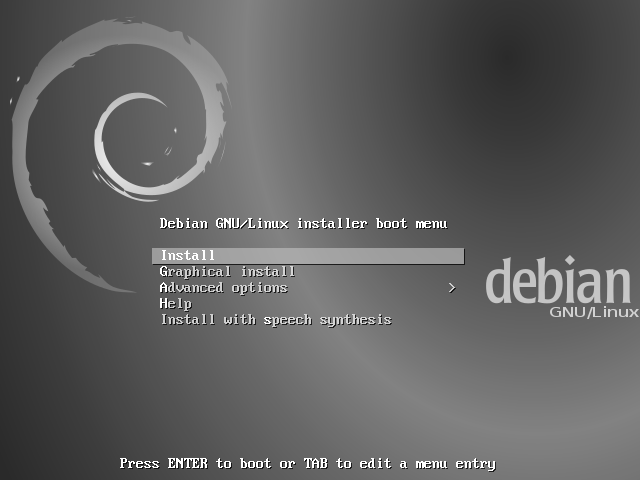
\includegraphics[width=0.8\hsize]{image201509/debian8-inst-01_mono.png}
 \end{center}
 \caption{インストーラ起動直後}
\end{minipage}
 \begin{minipage}{0.5\hsize}
  \begin{center}
   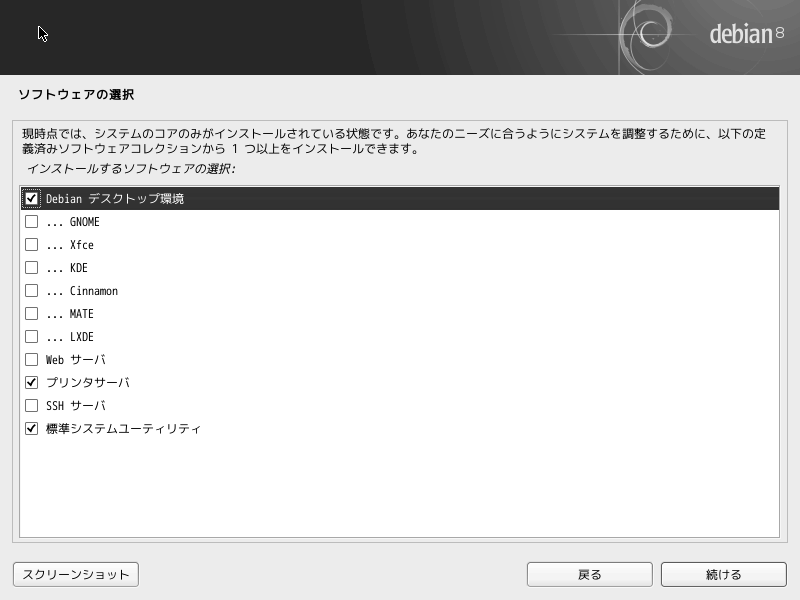
\includegraphics[width=0.8\hsize]{image201509/debian8-inst-02_mono.png}
  \end{center}
  \caption{グラフィカルインストール}
 \end{minipage}
\end{figure}

\begin{figure}[htbp]
 \begin{minipage}{0.5\hsize}
  \begin{center}
   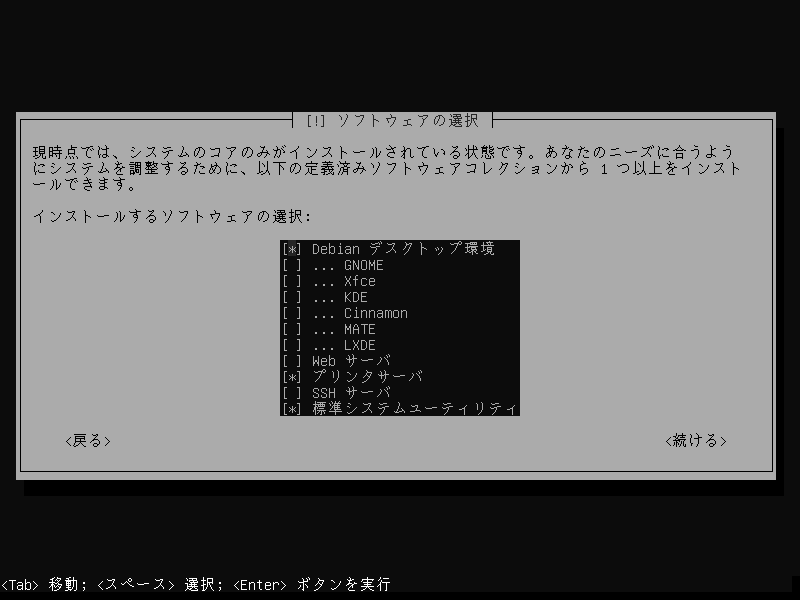
\includegraphics[width=0.8\hsize]{image201509/debian8-inst-03_mono.png}
  \end{center}
  \caption{テキストインストール}
 \end{minipage}
 \begin{minipage}{0.5\hsize}
  \begin{center}
   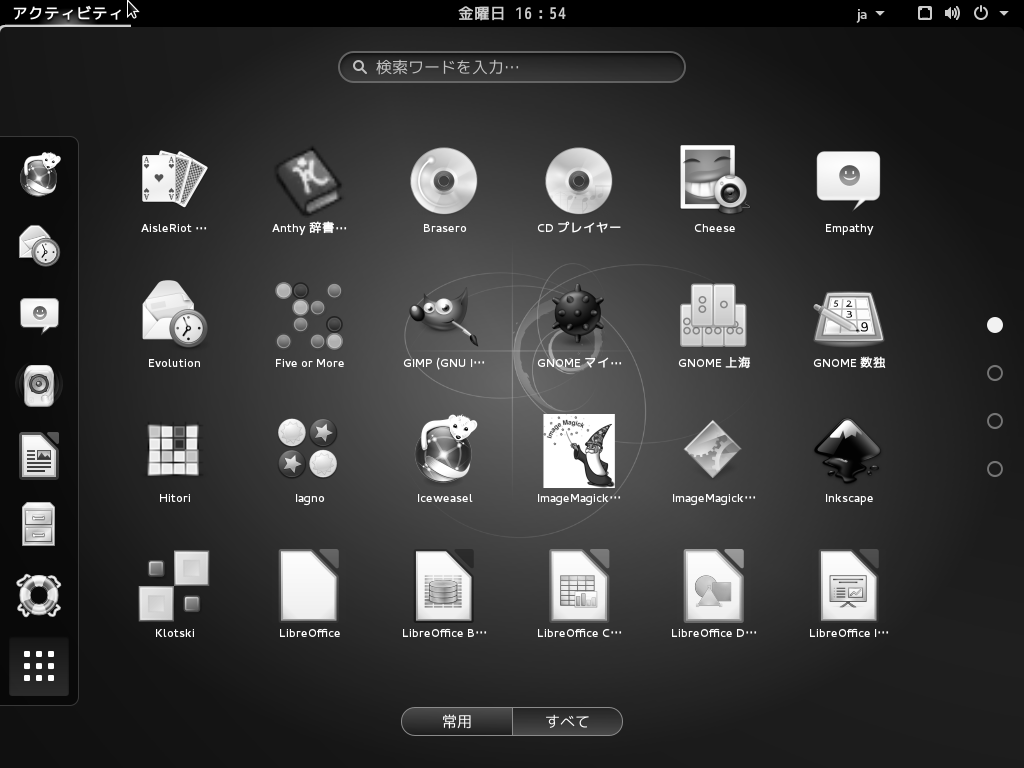
\includegraphics[width=0.8\hsize]{image201509/debian8-gnome_mono.png}
  \end{center}
  \caption{GNOME環境}
 \end{minipage}
\end{figure}

\begin{figure}[htbp]
 \begin{minipage}{0.5\hsize}
  \begin{center}
   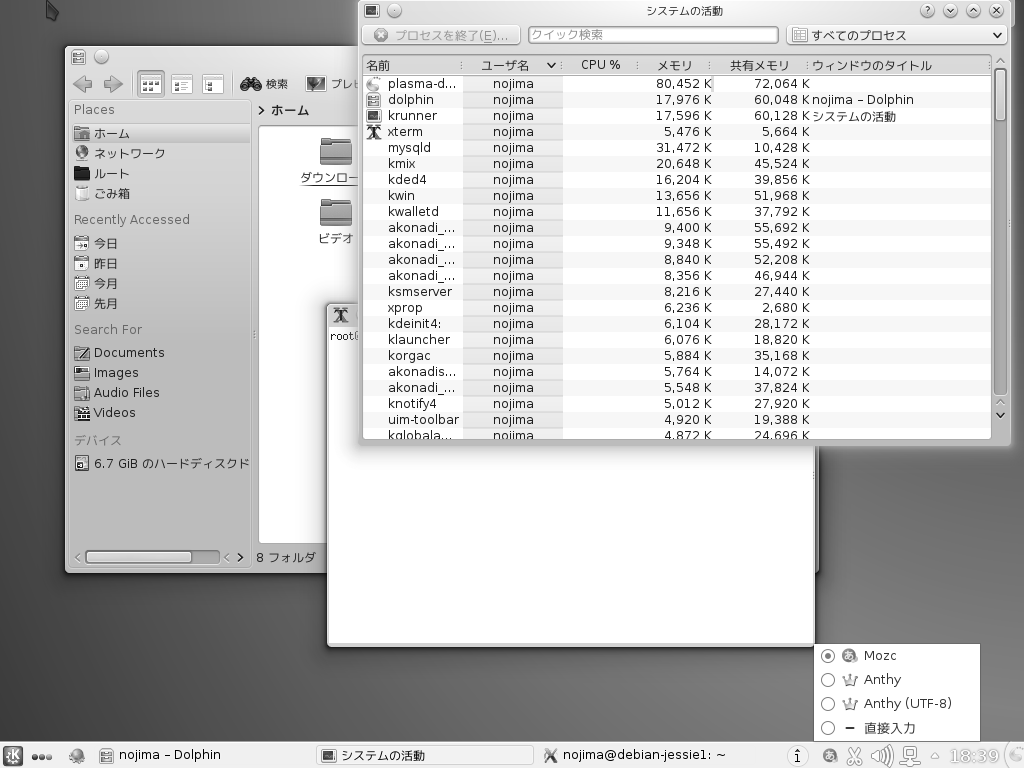
\includegraphics[width=0.8\hsize]{image201509/debian8-kde_mono.png}
   \caption{KDE環境}
  \end{center}
 \end{minipage}
 \begin{minipage}{0.5\hsize}
  \begin{center}
  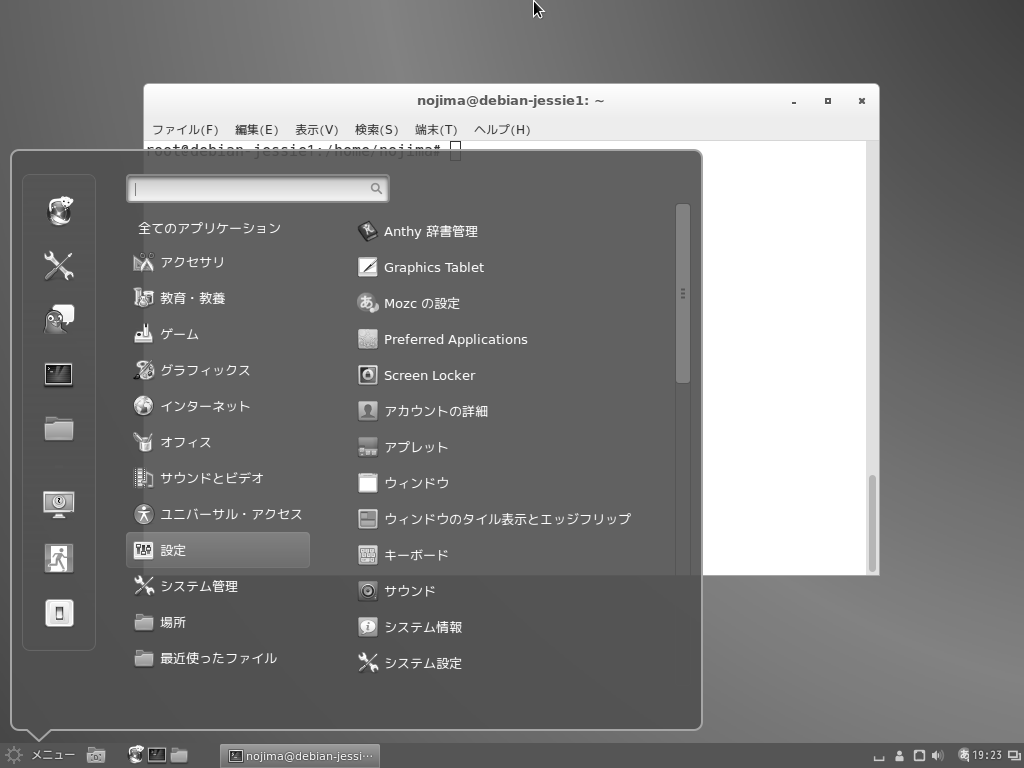
\includegraphics[width=0.8\hsize]{image201509/debian8-cinnamon_mono.png}
  \caption{cinnamon環境}
  \end{center}
 \end{minipage}
\end{figure}

\clearpage

\subsection{リリースその他}
  \begin{center}
    \Large
2015年4月30日 Debian GNU/Hurd 2015リリース
  \end{center}

\begin{itemize}
\item GNU Hurd 0.6ベース
\item GNU Mach 1.5搭載
\item とりあえずの動作なら、仮想環境で試せます。是非お試しあれ。
\end{itemize}


\subsection{Debian GNU/Hurd 2015 Live}

  Liveイメージもあるよ!\\
\url{https://www.gnu.org/software/hurd/hurd/running/debian.html}から抜粋

\begin{commandline}
# wget http://people.debian.org/~sthibault/hurd-i386/debian-hurd.img.tar.gz
# tar xz < debian-hurd.img.tar.gz
# kvm -m 512 -drive cache=writeback,file=debian-hurd-20150320.img
\end{commandline}
  

\subsection{Debian GNU/Hurd 2015 Live}

Debian GNU/Hurd 2015 Liveの様子。

\begin{center}
 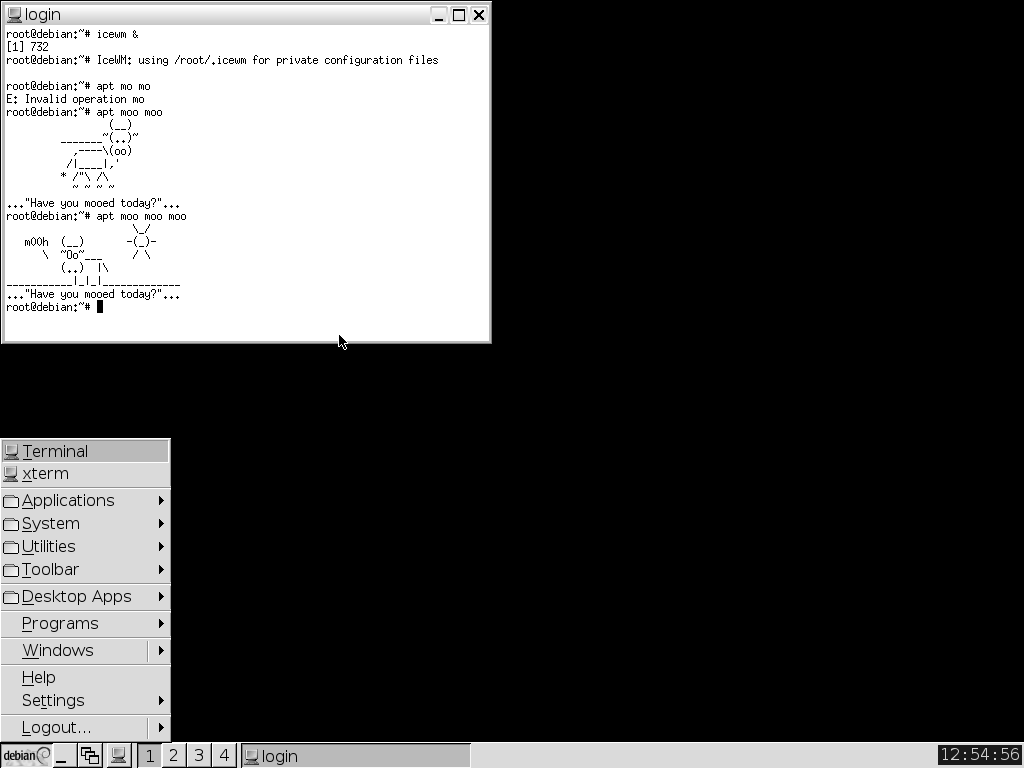
\includegraphics[width=0.9\hsize]{image201509/gnu-hurd-live_mono.png}
\end{center}
 
\subsection{次期バージョンのコード名}

  \begin{itemize}
  \item Debian 9 Stretch ←次回リリース
  \item Debian 10 Buster ←次々回リリース
  \end{itemize}
  

\subsection{Stretchスケジュール(予定)}

以下はStrechの開発に関する予定:

\begin{itemize}
  \item 2016年9月5日 Transition Freeze
  \item 2016年11月5日 Soft Freeze
  \item 2016年12月5日 Freeze
\end{itemize}

参照 DebConf15のリリースチームの動画:
\url{http://caesar.acc.umu.se/pub/debian-meetings/2015/debconf15/Onwards_to_Stretch_and_other_items_from_the_Release_Team.webm}

 なお、Freezeはリリースの事ではないので注意。Strechに搭載する新規のパッケージの受付を完全にやめ、RCバグ潰しに専念しますという意味。
  

\subsection{gcc-5/libc++6 移行作業中}

 現在、開発版(sid)では、Stretchにて新しいバージョンのコンパイラでパッケージを構築できるようにするため、一旦gcc-5系列及び、libc++6の元でバイナリビルドできるようにする大作業が行われています。

\begin{itemize} 
\item ABIレベルで変更
\item C++11対応
\item GFortranでコンパイルするパッケージもこちの影響を受ける
\end{itemize}


\subsection{httpredir.debian.org稼働開始}

 ネットワーク観点から、もっとも近いdebianのmirrorサイトを紹介するサービスであった、
\begin{itemize}
  \item cdn.debian.net ... DNSクエリで、もっとも近いmirrorサイトを返す
  \item http.debian.net ... http redirectを使って、もっとも近いmirrorサイトを返す
\end{itemize}
が終了し、代わりのサービスとして、正式に httpredir.debian.orgが稼働しました。
\\
  が、しかし本来、
  \begin{commandline}
# cat /etc/apt/souces.list
deb http://httpredir.debian.org/debian/ jessie main
deb-src http://httpredir.debian.org/debian/ jessie main
deb http://httpredir.debian.org/debian/ jessie-updates main
deb-src http://httpredir.debian.org/debian/ jessie-updates main
#
  \end{commandline}
で、うまく近いmirrorが紹介されるはずが、何故か日本は精度が悪い状況です。インストーラによって設定されるftp.jp.debian.orgの方が現在は良いです。

%201506tokyo
%-------------------------------------------------------------------------------
\dancersection{Debianと脆弱性対応のあれこれをまとめてみた}{野島 貴英}
%-------------------------------------------------------------------------------

\subsection{はじめに}

 コンピュータセキュリティの勉強会にて登壇を頼まれました。ちょうど良かったので、Debianの脆弱性対応をおさらいして、発表してみることにします。

\subsection{Debianのセキュリティチーム}

 Debianパッケージの脆弱性問題を専門に扱っている心臓部のチームの連絡先は以下の通りです。

\begin{itemize}
\item security@debian.org または 
\item team@security.debian.org
\end{itemize}

\subsection{脆弱性に関するML}

 Debianの脆弱性に関するアナウンス・議論が行われているMLは次のとおりです。

 \begin{itemize}
 \item  Debianパッケージのセキュリティに関するアナウンス\\
debian-security-announce@lists.debian.org\\
アーカイブ:\\
\url{https://lists.debian.org/debian-security-announce/}
 \item  Debianパッケージの脆弱性に関するオープンな議論\\
debian-security@lists.debian.org\\
アーカイブ:\url{https://lists.debian.org/debian-security/}
 \end{itemize}

\subsection{脆弱性対応が行われないアーカイブエリア}

 Debianパッケージ群は、main/contrib/non-freeのアーカイブエリアでそれぞれ提供されています。実は、脆弱性対応について、contrib/non-freeのアーカイブエリアのパッケージについては、基本的に除外されています。

 こちらの理由としては、contribとnon-freeに収められたソフトウェアのライセンスの問題によります。これらのソフトウェアはライセンスの都合上、勝手に直すことが許諾されていない場合があるためとなります。もちろん、contribとnon-freeであっても、ライセンス上、直しても良いものもあり、こちらについては通常の通りセキュリティチームにて脆弱性対応が図られることがあります。

\subsection{脆弱性に関しての対応の流れ}

 DebianユーザあるいはDebianの関係者にかかわらず、もし脆弱性の問題を見つけたら、
\begin{description}
\item [PAT1:] 既知の問題(公開済脆弱性情報)の場合は、securityタグをつけてBTSしてください。
\item [PAT2:] 既知でない場合は、そっとsecurity@debian.org またはteam@security.debian.org にメールで連絡(英文)し、あとは指示に従えば良いです。
\end{description}

 もちろん、脆弱性対策パッチも書いたのであれば、報告の際にパッチも一緒に送ると喜ばれます。

\subsubsection{既知の脆弱性でない場合の動き}

 既知の脆弱性でない場合、セキュリティチームはDebian以外のベンダ(ディストリビューション等含む)関係者らにも脆弱性情報が共有され、CVEなどの脆弱性情報データベース登録にも協力する動きが取られます。

\subsubsection{既知の脆弱性の収集}

 Mitre社(CVEのDBを管理している会社)から、CVEの情報を定期的に取り込んでいます。こちらの情報に基づき、Debianに関係ある・なし、重要度を判定して仕分けされ、バグ追跡システムに登録していく仕組み(インフラ)があります。

\subsection{脆弱性対応状況の確認方法}

 以下のサイトで状況を確認できます。

 \begin{enumerate}
\item セキュリティ観点から確認したい場合
  \begin{itemize}
  \item \url{https://security-tracker.debian.org/tracker/}
  \item 様々な視点から、巷の脆弱性データベースとDebianの各パッケージの対応状況を確認可能です。
  \end{itemize}
\item QA観点から確認したい場合
  \begin{itemize}
  \item \url{https://tracker.debian.org/}
     \item Debianパッケージについて、現在のバグの修正状況、パッケージのリリース状況がパッケージ毎にわかります。
  \end{itemize}
\item BTSした・されたものを確認したい場合
  \begin{itemize}
  \item \url{https://bugs.debian.org/}
  \item BTSした結果がどう扱われているか、進行しているか確認できます。
  \end{itemize}  
\end{enumerate}

 \subsection{その他トピック}

 以上で、まとめとしては終わったので、昨今のDebianのセキュリティに関するトピックをいくつか紹介します。

 \subsubsection{hardening}

  C/C++で書かれたプログラムについて、gccの機能を活用して、セキュリティ強化を行ったDebianパッケージを作る試みです。hardening有効時、ビルド時に実際に付け加えられるgccのオプションは以下の通りです。
  
\begin{commandline}
-fstack-protector-strong -Wformat -Werror=format-security -D_FORTIFY_SOURCE=2
\end{commandline}

 \subsubsection{Debianパッケージ済みの脆弱性静的解析ツール群}

  Debianでパッケージ済の脆弱性静的解析ツール群があります。

\begin{table}
\begin{center}
\begin{tabular}{|c|c|p{5cm}|}
\hline
項番 & パッケージ名 & 概要 \\ \hline \hline
1 & flawfinder & C/C++にてセキュリティ上問題の起きそうな部分を指摘。 \\ \hline
2 & rats & C, Perl, PHP, Pythonのコード上問題の起きそうな部分を指摘。\\ \hline
3 & pscan & C/C++にてformat文の文字列について問題の起きそうな部分を指摘。 \\ \hline
\end{tabular}
\end{center}
\caption{Debianパッケージ済み脆弱性静的解析ツール}
\end{table}

\subsubsection{lintian}

 lintianは、Debianパッケージについて、自動でスキャンして問題点を解析して警告してくれるツールであり、ある程度のセキュリティ対策の為の対応がパッケージ開発にあたり必須になっており、こちらが過不足なく行われているかをスキャンして開発者に教えてくれます。

 昨今にて搭載されたセキュリテイ対応の例として、梱包されているドキュメントにHTMLソースがあった場合、外部リンクが含まれているかをスキャンする事が追加されました。これは、もし、パッケージに含まれるドキュメントがHTMLであった場合に、外部リンクへアクセスするようなタグが混ざっているような事が無いようにします。もし、そういったタグやリンクが残っていると、ドキュメントをブラウザで開いた時に、うっかり悪意のあるサイトへ自動的に誘導されてしまうのを防ぎます。

\subsubsection{systemd}

 systemdにはセキュリティに関して強化を図ることが出来るオプションがいくつもあります。こちらをどう活かして、systemdの*.serviceファイルを作るかというお話です。
 
 良い文章として、「Security Features in systemd」\url{http://0pointer.net/public/systemd-nluug-2014.pdf}がありますので、見てみるとよいでしょう。

\subsubsection{Reproducible Builds}

 Debianの22,000を超えるソースパッケージを一旦再ビルドし、すでに配布されているDebianパッケージのバイナリと照合する試みの事です。こちらにより、Debianパッケージにいつの間にか悪意のあるバイナリが含まれているような事が無いかをチェックするのが狙いです。Debianの他にも、Fedora/OpenSUSE/NixOSでも行われているとのことです。

 詳しくは、
 \begin{description}
\item [Debian]
  \url{http://reproducible.alioth.debian.org/presentations/2014-02-01-FOSDEM14.pdf}

\item [Fedora]
   \url{http://securityblog.redhat.com/2013/09/18/reproducible-builds-for-fedora/}
 \end{description}

を参照ください。
   
\subsubsection{LTS(Long Time Support)}

Debianの各バージョンについて、セキュリティアップデートについてのサポート切れまでの期間を3年→5年へ延長する試みです。但し、数万もあるソフトウェア全部について5年もサポートするのは非現実的なので、限られたパッケージのセキュリティアップデートのみ延長します。

\begin{figure}[H]
\begin{center}
 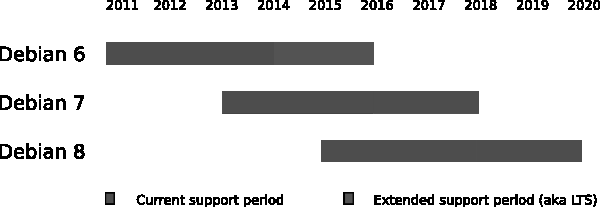
\includegraphics[width=0.7\hsize]{image201506/debian-lts-periods_mono.png}
\end{center}
\caption{LTSのサポート期間}
\end{figure}

 LTSは無料でも利用できる一方、有償サポート契約も用意されています。Freexian社と有償サポート契約を行うのですが、払った値段に応じて、サポートしてくれるパッケージの選択の要望が通りやすくなるという特典があるようです。日本の会社にて契約締結実績はGREE社があります。

 有償サポート契約について詳しくは「Debian Long Term Support」\url{https://www.freexian.com/en/services/debian-lts.html}を参照ください。

\subsubsection{debian-security-supportパッケージ}

 debian-security-supportパッケージを導入し、check-support-statusコマンドを実行すると、
現在お使いのDebian機に導入されいているパッケージの脆弱性のサポートについて、サポート切れ、もしくは、何らかの理由により脆弱性対策にあたり制限を加えざるを得なかったもののリストが取れるようになりました。

 このコマンドの動作としては、
\begin{itemize}
\item  /usr/share/debian-security-support/security-support-ended
\item /usr/share/debian-security-support/security-support-limited
\end{itemize}
に記載されたパッケージのサポート状況に関する制限の情報と、実際に導入されていてるパッケージ名を照合することにより動作します。もし、これらのファイルから、制限があるパッケージがマシンに見つかった場合は、警告を出してくれます。なお、LTSでは、どこまでパッケージについて、脆弱性対応のサポートがなされているかの確認ができます。

\subsection{おわりに}

 Debianの脆弱性対応についてまとめてみました。Debianのセキュリティ維持の為、様々な努力が払われていることがわかりました。

%201511 tokyo
%-------------------------------------------------------------------------------
\dancersection{Debian GNU/kFreeBSD セットアップガイド 2015年版}{杉本 典充}
%-------------------------------------------------------------------------------

\subsection{はじめに}

Debian GNU/kFreeBSDは、FreeBSDカーネルで動作するDebianです。Debianは単なるLinuxディストリビューションではなく、ユニバーサルオペレーティングシステムを目指しており、その例としてDebian GNU/kFreeBSDがあります。\footnote{私が知っている限り「Universal Operating System」という記述は本家webサイトトップページのtitleタグでしか見たことないです。}

ただDebian GNU/kFreeBSDはその特異さゆえにDebian GNU/Linuxと異なる点があります。今回は、Debian GNU/kFreeBSDに触れるにあたり、どのようにセットアップを行うとよいか説明します。

\subsection{Debian PortsとDebian GNU/kFreeBSD}

Debian Ports\footnote{\url{https://www.debian.org/ports/}}とは、さまざまなCPUやカーネルで動作するように移植を行うプロジェクトのことです。

FreeBSDカーネルで起動するDebianを作るプロジェクトがあり、そのDebianのことを「Debian GNU/kFreeBSD」と呼んでいます(kはkernelのこと)。現在ではIntel CPUのアーキテクチャのみあります(kfreebsd-amd64、kfreebsd-i386)。Debian 6 (Squeeze)ではテクノロジープレビューとして初めてstableリリースされました。Debian 7 (Wheezy)でも継続してstableリリースされたのですが、Debian 8 (Jessie)ではDropとなったためリリースされていません。\footnote{\url{https://lists.debian.org/debian-devel-announce/2014/09/msg00002.html} において、stableを維持しつつsidの開発を進めるにはそれなりに人手が必要であるが、kFreeBSDを作業する人手は不足していることが指摘されています。}


\subsection{Debian GNU/kFreeBSDのインストール}
\subsubsection{インストールイメージの入手}

\url{https://www.debian.org/devel/debian-installer/}にあるdaily-imagesを使ってインストールします。
kfreebsd-amd64版のmini.isoをダウンロードし、USBメモリにddしてインストールディスクを作成します。kfreebsd-i386版のmini.isoを利用しても構わないのですが、ファイルシステムにZFSを使う場合はメモリ不足になりがちなため注意してください。

mini.isoをddしたUSBメモリを差してPCを起動するとDebian Installerが起動します。なお、現時点のkfreebsd版Debian Installerは以下の制約があります。\footnote{本家FreeBSD-10.1のインストーラはUEFIブートに対応し、ディスク形式をGPTとしてインストールすることが可能です。}
\begin{itemize}
  \item UEFIブートに対応していない
  \item ディスク形式はMBRのみに対応している(GPTは非対応)
\end{itemize}


\subsubsection{インストーラの表示言語}

kfreebsd版Debian Installerは、日本語の表示ができません(インストーラでフレームバッファが有効になっていないと思われる)。そのため、LANG=Cでインストールを進めます。

\subsubsection{パーティション構成とファイルシステム}

Debian GNU/kFreeBSDをインストールするときはrootパーティションをMBRの基本パーティションにする必要があります(拡張パーティションにインストールするとgrubのインストールに失敗します)。swapパーティションは拡張パーティションに作成しても問題ありません。

この前提があるため、プリインストールのWindowsとデュアルブートしたい場合は、以下のパーティション構成でほぼ決まりになります。\footnote{ファイルシステムをUFSにする場合は基本パーティションの上限(4つ)を超えることがあるため、ディスク内のWindows用リカバリ領域を削除する、Dドライブを削除するなどの事前準備が必要になります。}

\begin{commandline}
# fdisk -l /dev/ada0
Disk /dev/ada0: 298.1 GiB, 320072933376 bytes, 625142448 sectors
Units: sectors of 1 * 512 = 512 bytes
Sector size (logical/physical): 512 bytes / 512 bytes
I/O size (minimum/optimal): 512 bytes / 512 bytes
Disklabel type: dos
Disk identifier: 0x33d61950

Device      Boot     Start       End   Sectors   Size Id Type
/dev/ada0p1 *         2048   2459647   2457600   1.2G  7 HPFS/NTFS/exFAT
  -> Windows 7のインストーラが自動で確保する領域
/dev/ada0p2        2459648 375142399 372682752 177.7G  7 HPFS/NTFS/exFA
  -> Windows 7のOSをインストールしたNTFSパーティション
/dev/ada0p3      580083712 625140399  45056688  21.5G  7 HPFS/NTFS/exFAT
  -> ノートPCメーカーのリカバリー領域
/dev/ada0p4      375142400 580083711 204941312  97.7G a5 FreeBSD
  -> Debian GNU/kFreeBSDをインストールするZFSストレージプール領域
  -> ZFSパーティションの中にrootボリュームとswapボリュームを作成します
\end{commandline}

4つの基本パーティションにうち、1つをZFSストレージプール(LVMの物理ボリュームに似ている概念)に割り当てます。そしてZFSストレージプールからrootボリュームとswapボリュームを作成します(別途bootボリュームを作成して/bootパーティションへ割り当てしなくても問題ありません)。

ディスクすべてをkfreebsdに割り当てることができ、かつメモリ搭載量が少ない環境(古いPCや仮想マシン)へインストールする場合はUFSを選択したほうがよいと思います。\footnote{インストール時に作成するUFSパーティションはsoft updateが無効になっています(つまり同期書き込みする設定になっている)。rescue modeから"tunefs.ufs -n enable "partition-path""を実行するとsoft updateを有効にして非同期書き込みに変更できますが、耐障害性が低下しますのでご注意ください。}

\subsection{Debian GNU/kFreeBSD固有のDebianパッケージ}

Debian GNU/kFreeBSD固有のパッケージの例を紹介します。

\subsubsection{kfreebsd-imageパッケージ}

Debian GNU/kFreeBSDのkernelイメージを収録したパッケージです。unstableにはkfreebsd-image-10.1があり現状のデフォルトkernelになっています。experimentalにはkfreebsd-image-10.2\footnote{FreeBSD-10.2は2015年8月14日 UTCにリリースされていますので次第にこちらがデフォルトになるでしょう。}、kfreebsd-image-11\footnote{現在のFreeBSD-CURRENTです。FreeBSD-CURRENTは、debianでいうところのunstableと似た位置付けであり、最新の開発版です。}もあります。

\subsubsection{zfsutilsパッケージ}

zfsutilsパッケージはZFSを操作するコマンドを含んだパッケージです。インストール時のファイルシステムにZFSを選択した場合はデフォルトでインストールされます。

kfreebsd-image-10.1で利用できるZFSのバージョンはver 28となっています。

\begin{commandline}
  $ zpool upgrade -v
  (snip)
  28  Multiple vdev replacements
\end{commandline}

\subsubsection{freebsd-utilsパッケージ}

FreeBSD固有のコマンドを含んだパッケージです。/sbin/mount\_*、/usr/sbin/jailなどが入っています。

\subsubsection{freebsd-smbfsパッケージ}

freebsd-smbfsパッケージは、Windowsファイル共有(SMB共有)へアクセスするためのパッケージです。
インストールすると、/usr/sbin/mount\_smbfsコマンドが使えるようになります。

Windowsファイル共有先をmountするには以下のコマンドを実行します。

\begin{commandline}
# mount_smbfs -E UTF-8:CP932 -I {ファイルサーバのIPアドレス} -U {smbユーザ名} //{ファイルサーバのIPアドレス}/{dir} {mount先dir}
\end{commandline}

\subsubsection{freebsd-pppパッケージ}

freebsd-pppパッケージは、ダイアルアップする/usr/sbin/pppコマンドを含んでいます。3GやLTEに対応したUSBモデムを使う場合に必要となります。

Debian GNU/Linuxではpppパッケージやwvdialパッケージでダイアルアップしますが、kfreebsdでは使えないため注意が必要です。

ppp接続の例については後述します。

\subsubsection{pfパッケージ}

FreeBSD kernelがもつPacket Filterと呼ばれるいわゆるファイアウォール機能を制御するコマンド/sbin/pfctlを含んだパッケージです。\footnote{Linux kernelのnetfilter機能と制御コマンドiptablesに相当します。}

/sbin/pfctlの設定ファイルは/etc/pf.confであり、Linuxのiptables用設定ファイルと中身が全く異なります。

\subsection{WindowsとDebian GNU/kFreeBSDのデュアルブート設定}

Debian GNU/kFreeBSDのboot loaderはgrub2を利用しています。
grub2でDebian GNU/kFreeBSDとWindowsをデュアルブートしたい場合は以下の操作を行い、grubにメニューを追加します。((hd0,2)の部分はインストール環境に合わせて変更してください))

\begin{commandline}
  # cd /etc/grub
  # vi 40_custom.kfreebsd
  
  #!/bin/sh
  exec tail -n +3 $0
  # This file provides an easy way to add custom menu entries.  Simply type the
  # menu entries you want to add after this comment.  Be careful not to change
  # the 'exec tail' line above.
  menuentry ``Windows (loader)'' {
    insmod part_msdos
    insmod ntfs
    set root=(hd0,2)
    chainloader +1
  }

  # update-grub
\end{commandline}

\subsection{ハードウェアとソフトウェアのセットアップ}
\subsubsection{有線LAN}

有線LANは利用するドライバによってデバイス名が変化します(intelのPC向けならem0、realtekならre0)。
設定ファイルはDebian GNU/Linuxと同じ/etc/network/interfacesですが、allow-hotplug句はlinuxで使われるudevが提供している機能であることからkfreebsdでは利用できないため注意が必要です。

そのため、有線LAN接続環境がない状況でOSを起動すると有線LANによるDHCPのIPアドレス取得がタイムアウトするまでloginプロンプトが出てこなくなります(起動に時間がかかる)。私はノートPCにDebian GNU/kFreeBSDをインストールする場合は以下コマンドを手動で実行してネットワークへ接続するようにしています。

\begin{commandline}
  # vi /etc/network/interfaces

  #auto em0  <-コメントにします
  iface lan_home inet dhcp

  
  # ifup em0=lan_home
\end{commandline}

\subsubsection{無線LAN}

無線LANはThinkpad X220に搭載している「Intel Centrino advanced-N 6205」で動作することを確認しています。そのため、同じiwnデバイスと認識される「Intel Wireless WiFi Link 4965」以降のIntel製無線LANカードであれば動作すると思います。

無線LANを利用するためにkfreebsd-image-10系の最新版kernel、firmware、無線LANデーモン"wpasupplicant"をインストールします。\footnote{kfreebsdで無線LANが使えるようになったのは2014年8月頃と思われます。 \url{https://bugs.debian.org/cgi-bin/bugreport.cgi?bug=642468}}

\begin{commandline}
  # vi /etc/apt/sources.list

  deb http://ftp.jp.debian.org/debian/ unstable main contrib non-free

  # apt-get install kfreebsd-image-10-amd64
  # apt-get install firmware-iwlwifi wpasupplicant
  # reboot
\end{commandline}

FreeBSDの無線LANインタフェースは、物理インタフェースと論理インタフェースに分かれています。そのため、論理インタフェースを生成する必要があります。

\begin{commandline}
  # ifconfig iwn0  (これが物理インタフェース名)
  iwn0: flags=8802 metric 0 mtu 2290
  ether xx:xx:xx:xx:xx:xx
  media: IEEE 802.11 Wireless Ethernet autoselect (autoselect)
  status: no carrier
  nd6 options=23

  # ifconfig wlan create wlandev iwn0
  wlan0

  # ifconfig wlan0 (これが論理インタフェース名)
  wlan0: flags=8802 metric 0 mtu 1500
  ether xx:xx:xx:xx:xx:xx
  inet6 fe80::xxxx:xxxx:xxxx:xxxx%wlan0 prefixlen 64 scopeid 0x6
  ssid " channel 5 (2432 MHz 11g)
  country US authmode WPA2/802.11i privacy OFF txpower 15 bmiss 10
  scanvalid 60 bgscan bgscanintvl 300 bgscanidle 250 roam:rssi 7
  roam:rate 5 protmode CTS wme
  media: IEEE 802.11 Wireless Ethernet autoselect (autoselect)
  status: no carrier
      nd6 options=23
\end{commandline}
%" -- for emacs

接続する無線LANアクセスポイントの認証情報設定ファイルを作成します。

\begin{commandline}
  $ wpa_passphrase apname1 appassword > wpa_apname1.conf
  $ cat wpa_apname1.conf
  network={
    ssid=''apname1''
    #psk=''appassword''
    psk=e9fdcb43eba09b6342df30f14275625c8494e534799a82d6639b6124434ea627
  }  
\end{commandline}

無線LANアクセスポイントへ接続し、DHCPでIPアドレスを取得します。IPアドレスは論理インタフェースに付与されます。

\begin{commandline}
  # wpa_supplicant -i wlan0 -c ./wpa_apname1.conf
  Successfully initialized wpa_supplicant
  ioctl[SIOCS80211, op=20, val=0, arg_len=7]: Invalid argument
  ioctl[SIOCS80211, op=20, val=0, arg_len=7]: Invalid argument
  wlan0: Trying to associate with yy:yy:yy:yy:tt:tt (SSID='apname1' freq=2432 MHz)
  wlan0: Associated with yy:yy:yy:yy:yy:yy
  wlan0: WPA: Key negotiation completed with yy:yy:yy:yy:yy:yy [PTK=CCMP GTK=CCMP]
  wlan0: CTRL-EVENT-CONNECTED - Connection to yy:yy:yy:yy:yy:yy completed [id=0 id_str=]
  wlan0: WPA: Group rekeying completed with yy:yy:yy:yy:yy:yy [GTK=CCMP]

  # dhclient wlan0

  # /sbin/ifconfig wlan0
  wlan0: flags=8843 metric 0 mtu 1500
  ether xx:xx:xx:xx:xx:xx
  inet6 fe80::xxxx:xxxx:xxxx:xxxx%wlan0 prefixlen 64 scopeid 0x6
  inet 192.168.1.100 netmask 0xffffff00 broadcast 192.168.1.255
  ssid apname1 channel 5 (2432 MHz 11g) bssid yy:yy:yy:yy:yy:yy
  country US authmode WPA2/802.11i privacy ON deftxkey UNDEF
  AES-CCM 2:128-bit txpower 15 bmiss 10 scanvalid 60 bgscan
  bgscanintvl 300 bgscanidle 250 roam:rssi 7 roam:rate 5 protmode CTS
  wme roaming MANUAL
  media: IEEE 802.11 Wireless Ethernet OFDM/48Mbps mode 11g
  status: associated
          nd6 options=23
\end{commandline}

wpasupplicantコマンドで無線LANアクセスポイントへ接続を試みたがエラーが発生し接続できない場合があります。その場合は以下を試すと接続できる場合があります。

\begin{itemize}
  \item 接続先SSIDを2.4GHz帯のものに変更する。
  \item ``\texttt{\# ifconfig wlan0 -ht40}'' を実行する。\footnote{デュアルチャネル接続を無効にして、20MHz幅の電波で通信するように指示するコマンドです。}
\end{itemize}


\subsubsection{USBモデムによるダイアルアップ}

3GやLTEのUSBモデムを使ってダイアルアップ接続することができます。NTTドコモから出ている「L-02C」というLTEに対応したUSBモデムを例に接続する手順を説明します。

まずはpppコマンドとUSBモデム処理に使うコマンドをインストールします。

\begin{commandline}
  # apt-get install freebsd-ppp usb-modeswitch 
\end{commandline}

L-02CをPCに差すとCD-ROMデバイスとして認識します。そのため、L-02Cをモデムモードに変更するコマンドを実行します。

\begin{commandline}
  # vi /etc/usb_modeswitch.d/L02C.conf
  ########################################################
  # LG L-02C LTE modem

  DefaultVendor= 0x1004
  DefaultProduct=0x61dd

  TargetVendor= 0x1004
  TargetProduct=0x618f

  MessageContent=5553424312345678000000000000061b000000020000000000000000000000
  NeedResponse=1
  CheckSuccess=20

  # usb_modeswitch -c /etc/usb_modeswitch.d/L02C.conf
\end{commandline}

\begin{commandline}
  # ls /dev/cua*
  /dev/cuaU0.0       /dev/cuaU0.1       /dev/cuaU0.2       /dev/cuaU0.3
  /dev/cuaU0.0.init  /dev/cuaU0.1.init  /dev/cuaU0.2.init  /dev/cuaU0.3.init
  /dev/cuaU0.0.lock  /dev/cuaU0.1.lock  /dev/cuaU0.2.lock  /dev/cuaU0.3.lock
\end{commandline}

次にpppコマンドの設定ファイルを作成し、ppp接続します。利用する回線によって適時APN、ユーザ名、パスワードは変更してください。PPP接続に成功するとtunインタフェースが生成され、IPアドレスが付与されます。

\begin{commandline}
  # vi /etc/ppp/ppp.conf

  default:
    set log Phase Chat LCP IPCP CCP tun command
    ident user-ppp VERSION
    set device /dev/cuaU0.2
    set speed 38400
    set dial ``ABORT BUSY TIMEOUT 2 \
    \"\" \
    AT OK-AT-OK \
    AT+CFUN=1 OK-AT-OK \
    AT+CMEE=2 OK-AT-OK \
    AT+CSQ OK \
    AT+CGDCONT=1,\\\"IP\\\",\\\"apn.ne.jp\\\" OK \
    AT+CGACT? OK-AT-OK \
    AT+CGATT? OK \
    AT+CGCLASS? OK \
    AT+COPS? OK \
    ATD*99***1# CONNECT''
    set timeout 180
    enable dns

  myppp:
    set phone ``*99***1#''
    set authname ``apnuser''
    set authkey ``apnpass''
    set timeout 300
    disable ipv6
    set ifaddr 10.1.0.1/0 10.1.0.2/0 255.255.255.255 0.0.0.0
    add default HISADDR

  # ppp -foreground myppp
\end{commandline}

\subsubsection{ビデオドライバ}

現在、主流のビデオカードはIntel社のCPU内蔵グラフィックス、AMD社のRadeonシリーズ、NVIDIA社のGeForceシリーズがあります。
Debian GNU/kFreeBSDはFreeBSD向けに提供されるプロプラエタリドライバのビルド環境がないため、オープンソース版ドライバを利用する必要があります。そのため、Intel CPU内蔵グラフィックスまたはRadeonシリーズのビデオカードを利用することをおすすめします。\footnote{NVIDIA社ビデオカードを利用する場合、xserver-xorg-video-nouveauパッケージはLinux版のみの提供であるため使えず、オープンソース版ドライバxserver-xorg-video-nvは開発がすでに止まっておりかなり古いビデオカードしか対応してません。}

Intel CPU内蔵グラフィックスのビデオカードを利用する場合は以下のパッケージをインストールします。

\begin{commandline}
# apt-get install xserver-xorg-video-intel
\end{commandline}

Radeonシリーズのビデオカードを使用する場合は以下のパッケージをインストールします。

\begin{commandline}
# apt-get install xserver-xorg-video-ati
\end{commandline}

次はKMS(kernel mode settings)を有効にします。以下コマンドを実行するとコンソール画面の解像度が上がります\footnote{昔のkfreebsdでは、i915.koをloadしたままi915kms.koをloadするとrebootしてしまう現象が起こっていたため念のためunloadしています。現在のkfreebsd-image-10.1のkernelで試したところ、loadしたままでも大丈夫ではあるようです。}。KMSを有効にした状態にすると、X Window Systemで液晶モニタの解像度を最大限に利用でき、xrandrコマンドで外部モニタ出力もできるようになります。

\begin{commandline}
  # kldunload i915
  # kldload i915kms
\end{commandline}

再起動後も自動でkernel moduleをロードするように設定します。

\begin{commandline}
  # vi /etc/modules
  i915kms
\end{commandline}

\subsubsection{localeの再設定}

Debian InstallerではLANG=Cを選択してインストールしているため、出力メッセージが英語になっています。そのためlocaleを日本語に変更します。(ただし、コンソール環境では日本語メッセージが文字化けするので注意)

\begin{commandline}
  # dpkg-reconfigure locales

  -> ja_JP.UTF-8を選択する
\end{commandline}

\subsubsection{X Window Systemのキーボード設定}

FreeBSDのxorgではhalを使ってキーボードのレイアウトを自動判定しています。しかし、halはupstreamによるメンテナンスをすでに終了しており、kfreebsdでもdebianパッケージの提供は終了しています。そのためX Window System起動時のキーボードレイアウトはデフォルトの英語キーボードと判定されます。

キーボードレイアウトの変更はxorg.confで直接指定する、ウィンドウマネージャのキーボード設定を利用するなどして対応する必要があります。

\subsubsection{webブラウザ}

webブラウザはDebian GNU/Linux同様にiceweaselパッケージが提供されています。しかしchromiumパッケージはkfreebsdに存在しません。

またAdobe Flash PlayerはLinux用のバイナリとして提供されるため、Flashを見たい場合はgnashなどをインストールする必要があります(ただし動作の安定度は未知数)。

\subsubsection{USB 3.0}

kfreebsd-image-10-amd64パッケージのkernelにおいて、xhci.koがstatic linkされていることを確認しています。ただし、USB 3.0をもつPCにDebian GNU/kFreeBSDをインストールしたことがないため動作は未確認です。

\subsubsection{サウンドドライバ}

FreeBSDはOSSという仕組みでサウンドを出力します(ALSAはLinux専用のサウンドシステムです)。最近のPCにはHigh Definition Audio規格のチップが搭載されることが多いため、snd\_hda.koドライバでサウンドを出力することができます(snd\_hda.koはkernelにstatic linkされています)。

また、pulseaudioパッケージをインストールし、audaciousを使ってpulseaudio経由で音楽を再生できることは確認しています。

\subsubsection{電源関係}

CPUクロックの制御はpowerdパッケージのpowerdが行っています。現在動作中のCPUクロック数はsysctlコマンドで取得できます。

\begin{commandline}
  $ sysctl dev.cpu.0.freq
  dev.cpu.0.freq: 800
\end{commandline}

バッテリー残量を取得するにはacpiconfコマンドを実行します。

\begin{commandline}
  $ /usr/sbin/acpiconf -i 0
  Design capacity:62160 mWh
  Last full capacity:26300 mWh
  Technology:secondary (rechargeable)
  Design voltage:11100 mV
  Capacity (warn):1315 mWh
  Capacity (low):200 mWh
  (snip)
  State:discharging
  Remaining capacity:95%
  Remaining time:1:25
  Present rate:17681 mW
  Present voltage:12186 mV
\end{commandline}

サスペンドとハイバーネートについては未確認です。

\subsubsection{USBメモリのmount}

FreeBSDではUSBメモリをPCに差すと/dev/da0s1のように認識します。FAT16またはFAT32の領域をもつUSBメモリを/mnt/usbへmountするには以下のコマンドを実行します。

\begin{commandline}
# mount_msdosfs -L ja_JP.UTF-8 -D CP932 /dev/da0s1 /mnt/usb
\end{commandline}

exFATをmountするのはexfat-fuseパッケージを、NTFSをmountするにはntfs-3gパッケージを使うと思われますが、試したところどちらもエラーが出てmountできませんでした。

\subsubsection{Linuxエミュレーション}

FreeBSD kernelにはlinuxバイナリ互換機能があり、Linuxのi386バイナリを実行することができます。\footnote{FreeBSD kernelのkernel moduleであるlinux.koが処理しています。}

debootstrapでlinux-i386環境を用意しchrootすることによってlinux-i386形式のバイナリを実行することができます。この機能を使うことによりlinuxバイナリのみ提供されるソフトウェアをkfreebsd上で利用することができます。\footnote{本家Java、Adobe Flash Player、Adobe Readerなどが該当します。}。

\subsubsection{仮想化}

FreeBSDにはFreeBSD Jailというコンテナ型仮想化環境を実行する機能があります。freebsd-utilsパッケージをインストールすることで利用できます。\footnote{本原稿の発表当時(2015年11月)はjlsコマンド、jexecコマンドがまだありませんでしたが、その後bugfixされて使えるようになっています。 \url{https://bugs.debian.org/cgi-bin/bugreport.cgi?bug=806562}}

Debian GNU/kFreeBSDにqemuパッケージはありますので、他のOSを使う必要がある場合は利用してもよいでしょう。(ただしあまり使ったことがないため、動作の安定度は未知数)

その他にFreeBSDにはOSを完全仮想化して動作させるvirtualbox、bhyveがありますが、Debian GNU/kFreeBSDにはまだ移植されていません。

\subsection{おわりに}

Debian GNU/kFreeBSDのインストール方法とセットアップ方法について説明しました。動作確認ができていない機能や移植されていない機能もまだ多くありますが、OSを開発したい方にはよい腕試しの場になると思います。興味のある方はまず使ってみるところから始めるのはいかがでしょうか。

\subsection{参考文献}

\begin{itemize}
  \item 「Debian\_GNU/kFreeBSD - Debian Wiki」 \url{https://wiki.debian.org/Debian_GNU/kFreeBSD}
  \item 杉本典充 (2015). 「Debian GNU/kFreeBSDにおけるJail構築を試してみた」 \url{http://tokyodebian.alioth.debian.org/pdf/debianmeetingresume201502-presentation-sugimoto.pdf}
\end{itemize}

%201508 tokyo
%-------------------------------------------------------------------------------
\dancersection{APT1.1 超☆牛さんパワー炸裂!}{野島 貴英}
%-------------------------------------------------------------------------------

\subsection{はじめに}

 debian-devel-announceに、''Moo! 9th preview of APT 1.1 released: Go and test new supercow powers''というタイトルで、APT 1.1のアナウンスが流れました。

 今回は、Debianの重要なツールの1つであるAPTについて、1.1に搭載された特徴をネタにして、いろいろ調べてみました。

\subsection{Debconf15のセッション}

 2015/8/15-8/22で開催されたDebconf15のセッションで、APT1.1のセッションが開かれました。こちらビデオが公開されていますので、興味ある方は是非ご覧ください。

 ビデオ:''This\_APT\_has\_Super\_Cow\_Powers''\\
 \url{http://meetings-archive.debian.net/pub/debian-meetings/2015/debconf15/This_APT_has_Super_Cow_Powers.webm}

\begin{figure}[H]
\begin{center}
 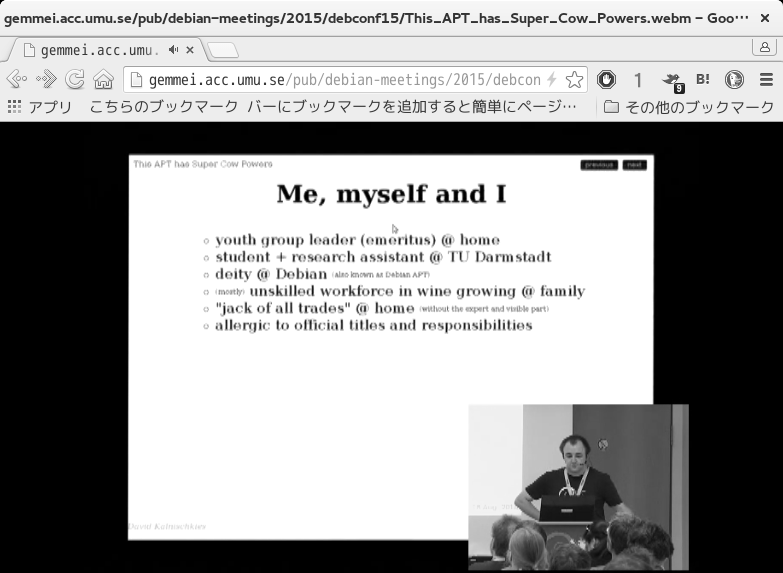
\includegraphics[width=0.5\hsize]{image201508/debconf15-apt_mono.png}
\end{center}
\caption{Debconf15のAPT1.1のセッションの様子}
\end{figure}

\subsection{APT 1.1を評価してみる}

 2015/8/22現在、APT 1.1はexperimentalリポジトリにあります。早速、試して見たい方は以下のようにすることで導入できます。

\begin{commandline}
$ sudo vi /etc/apt/source.lists
deb http://ftp.jp.debian.org/debian/ experimental main contrib non-free
deb-src http://ftp.jp.debian.org/debian/ experimental main contrib non-free
$ sudo apt-get update
$ sudo apt-get -t experimental install apt
$ apt
apt 1.1~exp9 (amd64)
Usage: apt [options] command
...中略...
 full-upgrade - upgrade the system by removing/installing/upgrading packages
 edit-sources - edit the source information file
\end{commandline}

 手元のDebian sid環境に導入してしばらく使っていますが、特に動作に問題は見当たりませんでした。apt update,apt full-upgrade, apt autoremoveなど一通りの動作は問題なくできており、致命的なバグにも特に遭遇していません。是非お試しあれ。

\subsection{APT 1.1の特徴}

 jessie搭載のAPT 1.0.9.8に比べての違いを述べてみます。

 先に紹介したDebconf15のビデオによれば以下の点が違いとなります。

\begin{itemize}
\item リポジトリの情報のセキュリティ検証が強化された。
\item deb822形式でリポジトリを指定するやり方にて機能強化。(/etc/apt/*.sourcesファイル)
\item httpredir.debian.orgを受けて、処理の途中経過の表示を変更。
\item Pinningがちゃんと動くようになった。
\item 依存関係をする場合、ローカルにおいた.debファイルを直接指定してもインストールでき、ソースビルドの依存関係を指定する方法が柔軟になった。
\end{itemize}

 まずは、man apt、man apt-getで記載されている内容で、トピックを絞って違いを紹介します。

\subsubsection{apt autoremove}

 APT1.1に搭載されたaptコマンドのautoremove命令について説明します。

 何かパッケージをインストールした場合、依存関係を満たすためだけにインストールされたパッケージが過去にあるとします。ここで、現在はその依存関係からも外されており、もはや全く使われていないパッケージがあります。このコマンドをつけてaptコマンドを起動すると、こういった使われていないパッケージを削除することが出来ます。

\begin{commandline}
$ sudo apt autoremove
\end{commandline}
%$

\subsubsection{autoremove仕組み}

 autoremoveはどのようにして消去すべきパッケージを見つけるのでしょうか?

 依存関係が見当たらないパッケージの中には、利用者が自分で明示して入れたパッケージもあります。そのため、必ずしも他のパッケージで依存していないということだけを条件にして、autoremoveでパッケージを消すようなことは避けなければなりません。autoremoveにより、自動で消去して良いパッケージを判断する基準は次の通りです。
 
\begin{description}
 \item [Step 1.] /var/lib/apt/extended\_statesファイルの記録に、過去、依存関係を満たすためにパッケージを導入したかどうかの記録である''Auto-Installed: 1''と記されているパッケージを消去の候補とする。
 \item [Step 2.] すでにインストール済パッケージのどれからも依存関係に無いかどうか?
 \item [Step 3.] さらに、
\begin{itemize}
\item Recommendsとして提案されているパッケージはインストールして欲しいと明示した場合、
\item Suggestとして提案されているパッケージはインストールして欲しいと明示した場合、
\end{itemize}
のいずれにも該当していないか?
\end{description}

以上のStep 1.〜3.の判断を経たパッケージが、自動で消去して良いパッケージとして扱われます。

\subsubsection{man apt-getとの違い}

次にman apt-getで見た1.0.9.8との違いについて紹介します。

 \begin{itemize}
\item \texttt{indextargets} \\
   apt-get updateで更新されるファイルと状態をdeb822形式で表示します。
 \item \texttt{--allow-downgrades} \\
   特定パッケージをダウングレードすることにより依存関係が満たせるときに、ユーザに尋ねず実行してまうというオプションです。
 \item \texttt{--allow-remove-essential} \\
   何らかの理由によりDebianシステムの必須パッケージ(essentialパッケージとして分類されている)ものを消せば依存関係が満たせるときに、消してよいか?を尋ねず消してしまうオプションです。
 \item \texttt{--allow-change-held-packages} \\
  何らかの理由によりHold扱いにしたパッケージを削除すれば依存関係が満たせるときに、消してよいか?を尋ねず消してしまうオプションです。
 \item \texttt{--no-allow-insecure-repositories} \\
   リポジトリにあるReleaseファイル(InReleaseファイル)のGPGによる署名が確認出来ない等、セキュリティ上問題があるとみなされたリポジトリが含まれた場合、apt-get update操作を失敗させます。
 \end{itemize}
 
 \subsubsection{リポジトリ堅牢化}

 APT 1.1はリポジトリのセキュリティの正当性評価が強化されています。正当性評価の元となるファイルにReleaseファイル(InReleaseファイル)があります。

\begin{commandline}
$ curl http://cloudfront.debian.net/debian/dists/unstable/InRelease
-----BEGIN PGP SIGNED MESSAGE-----
Hash: SHA256

Origin: Debian
Label: Debian
...中略...
MD5Sum:
 e9f9b477f2430a7d0e2dd686da1af507 30975818 Contents-amd64.gz
 d158f809191a841bedf9ff50e34e0ebe 30421142 Contents-armel.gz
...中略...
-----BEGIN PGP SIGNATURE-----
Version: GnuPG v1

iQIcBAEBCAAGBQJV1+IMAAoJEItIrWJGklVTgloP/0+XAch/TMtTSfH+N1QFl+q2
Woas1LpWhHDO12U6vuPq5wghCPYE5ctNuDxFtTy9j01lsf6kWXPDh1QupNENDNHr
lfZ7Qa9gFr8W3tH1tnPwsSqcQmu9bMkR0sRDVSfcFlDioVhN/h+jWW7j7J7nrZrE
...中略...
\end{commandline}
   
InReleaseファイルを見るとわかるとおり、

\begin{itemize}
\item リポジトリに含まれる様々なファイルは全てmd5sum付きでInReleaseファイルに記録
\item さらにInReleaseファイルも電子署名による正当性確認が出来るようになっている
\end{itemize}

となります。

 今回APT1.1では、基本的にInReleaseファイルの無い、あるいは、他に必要なファイルが欠落しているなど、セキュリティ観点からの正当性確認が出来ないリポジトリは取り扱いを完全にやめる設計にしたとのことです。

\subsubsection{httpredir.debian.org対応}

 2015/5月頃、Debianユーザに最も近いmirrorサーバーをHTTP Redirectでaptに教えてくれるサービスが稼働しました。つまり、ユーザは/etc/apt/sources.listに、httpredir.debian.orgを指定すれば、ユーザに最も近いmirrorサーバーへリダイレクトされます。

 ここで、リダイレクトされた結果どこのサーバから取得するのか?がわかると便利な事が多いです。このため、APT1.1のapt/apt-getはリダイレクトされた先の情報を表示するように変更されました。

\subsubsection{参考:httpredir.debian.orgの様子}

 httpredir.debian.orgが何を返却するのかを以下に示します。

\begin{commandline}
$curl -v http://httpredir.debian.org/debian/dists/sid/InRelease
> GET /debian/dists/sid/InRelease HTTP/1.1
> Host: httpredir.debian.org
> User-Agent: curl/7.44.0
> Accept: */*
> 
< HTTP/1.1 302 Found
< Date: Sat, 22 Aug 2015 03:54:12 GMT
< Location: http://cloudfront.debian.net/debian/dists/sid/InRelease
< Content-Type: text/plain
...省略...
\end{commandline}    

 見てのとおり、cloudfront.debian.netにリダイレクトが指示されるのが確認できると思います。

{ \scriptsize
 \begin{itembox}[l]{cloudfront.debian.net?}
 前ページのリダイレクト先にて、
\url{http://cloudfront.debian.net/}
とリポジトリが提案されています。これは、2年前にdebian-cloudチームでアナウンスがあった、AWSのcloudfrontというCDNの仕組みを使ってデータ配布を行う試みのリポジトリです。
(\url{https://lists.debian.org/debian-cloud/2013/05/msg00066.html})

 もともと、CDNはユーザに最も効率的なサーバを提示してデータを配る仕組みであり、
AWSのcloudfrontは相当な規模とサービスエリアを持つCDNサービスですので、
そもそもこちらがあるなら、AWSのサービスがカバーしている国では、httpredir.debian.orgを使わなくてすみそうな気もします。しかしながら、ソフトウェア自由をモットーとするDebianとしては、一企業のサービスに依存しないようにすることが重要ですので、Debianとしては、httpredir.debian.orgを維持・運用する必要があります。
 \end{itembox}
}

\subsection{deb822形式}

 APT 1.1では、deb822形式でリポジトリを指定するやり方にて機能強化が図られました。ここでは、deb822形式とはどんなものかを紹介します。

 APT1.1が手元にあれば、簡単にdeb822形式でリポジトリの情報を表示させる事が出来ます。

\begin{commandline}  
$ apt-get indextargets
MetaKey: main/source/Sources
ShortDesc: Sources
Description: http://ftp.jp.debian.org/debian sid/main Sources
URI: http://ftp.jp.debian.org/debian/dists/sid/main/source/Sources
Filename: /var/lib/apt/lists/ftp.jp.debian.org_debian_dists_sid_main_source_Sources
Optional: no
Codename: sid
...中略...
\end{commandline}  
  
 出力されるフォーマットを見るとわかるのですが、RFC822ヘッダの形式によく似ています。ここから、deb822と名前を取ったようです。

  特徴として、RFC822と同様ですので、ヘッダを増やせば、簡単に機能拡張できるという点が上げられます。

  また、動作未確認ですが、DebConf15のビデオによれば、
\begin{quote}
  /etc/apt/source.list.d/xxxx.sources
\end{quote}
(末尾が、.sourcesである事が必要)という名前でdeb822形式で置いておくと、
こちらをsources.listに指定したのと同様の動作をapt/apt-getは行うとのことです。
  
\subsection{牛さんパワー健在!}

 APT 1.1にも ``moo'' 命令は健在です。息抜きに、こちらを紹介しておきます。

 man aptには記載の無いオプションですが、以下にaptの場合の起動方法を載せます。

\begin{commandline}  
$ apt moo 
$ apt moo moo [--color]
$ apt moo moo moo  
$ faketime '1997-04-01' apt moo
\end{commandline}    

\begin{figure}[H]
\begin{center}
 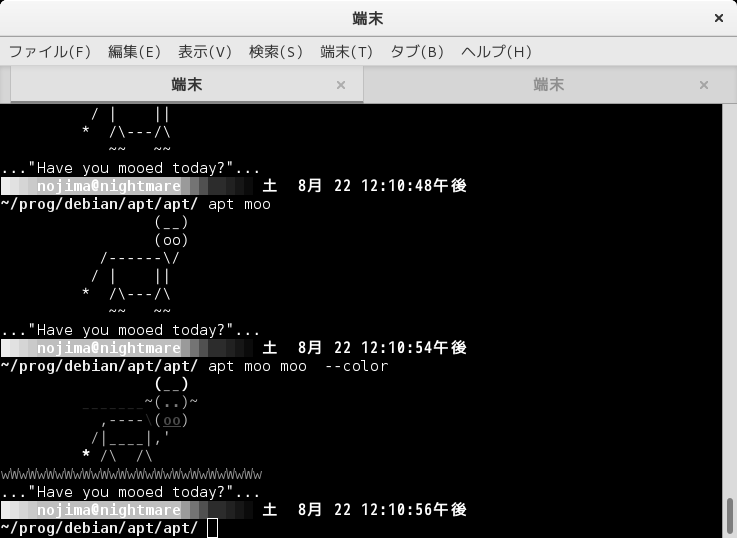
\includegraphics[width=0.7\hsize]{image201508/apt-moo_mono.png}
\end{center}
\caption{apt mooコマンド結果例}
\end{figure}

 実行するとわかるのですが、ASCIIキャラクタで描画された各種の牛の絵が表示されます。

\subsection{おわりに}

 まだまだ、APT1.1について、今回ここでは書ききれない程の変更が加えられているようですが、このへんにしておきます。実際、gitで落として差分を確認しましたが、実に2万行を超える変更が行われていました。正式リリースになって、ドキュメントも充実すると良いですね。
   
%201507tokyo
%-------------------------------------------------------------------------------
\dancersection{DebianでHTTP/2を試す}{野島 貴英}
%-------------------------------------------------------------------------------

\subsection{はじめに}

 2015/5にHTTP/2がRFC7540として遂に文章化されました。また、最近でも、ほうぼうでWEBページあるいはサービスについて、HTTP/2の対応度合いについて聞かれるようになってきました\footnote{某有名携帯電話イベントでHTTP/2をアプリ開発者に全力推奨している件を見て慌てたりしたのは秘密...}。

 ここでは、Debianで、HTTP/2の環境をちょっと作って試してみました。

\subsection{ところでHTTP/2って?}

  WEBブラウザがサーバと通信する際に、HTTP/1.x(xは0,1の数字)が長年(HTTP/1.1は15年以上も!)使われています。しかしながら、昨今のWEBページは、HTTP/1.xが策定された頃に比べて格段にリッチなページとなっており、1ページを表示する為に必要な通信量は格段に増えています。HTTP/1.xのままでは、WEBの通信が非効率となってしまいました。

 HTTP/1.1の欠点を克服するために、google社でSPDYが開発され、さらにSPDYを参考にして、沢山の人の貢献により、次世代のHTTP通信規格が策定されました。これがHTTP/2となります。

 \subsection{HTTP/2の特徴}

 HTTP/2の特徴としては以下の通りです\cite{ref:http-2-faq}。
 
\begin{itemize}
\item テキスト電文ベースではなく、バイナリ電文を使います。
\item 1本のTCPコネクション上で、複数のリクエスト・レスポンスを多重化してやりとりできるように設計されています。
\item  リクエスト・レスポンスに使われるヘッダ情報を無駄の無い電文にし、さらに圧縮し、より効率的に通信できるようにしています。実はモバイル端末などでは、パケットの往復にかかる時間が長いので、リクエスト・レスポンスの開始1パケット目にできるだけ情報を詰め込むことは通信時間を縮めるのに非常に有効です。
\item 1つのリクエストで、ブラウザが続けて必要とするデータをまとめてレスポンスできる機能が入りました(サーバプッシュという機能。)\cite{ref:server-push-primer}
 \end{itemize}

\subsection{HTTP/2さらに詳しく}

  これ以上HTTP/2プロトコルについて、詳しく調べたい人は、

 \begin{itemize}
  \item HTTP/2本家\\
    \url{https://http2.github.io/}
  \item 高速・大規模ネットワーク時代に向けて改良されたHTTP/2プロトコル
    \url{http://www.atmarkit.co.jp/ait/articles/1409/18/news135.html}
  \item twitterの\#http2studyタグ
  \item http/2 Advent Calender 2014
    \url{http://qiita.com/advent-calendar/2014/http2}
\end{itemize}

 などなど、多数の良い解説がありますので是非ご覧ください。これ以上細かいHTTP/2のプロトコル仕様についてはここでは割愛します。

 \subsection{HTTP/2の良いデモサイト}

 論より証拠で、HTTP/2が優れているか?を試せる非常に良いデモサイトがあります。是非お試し下さい。なお、Debian sidのchromium/iceweaselで動作確認を確認できています。
 \\
\begin{center} 
 \url{https://http2.golang.org/gophertiles}
\end{center}

\subsection{HTTP/2の通信開始の仕方}

 HTTP/2を使ってブラウザからアクセスするとき、現状、TLSのALPN/NPNでHTTP/2を指定して、やりとりを開始するやり方しか現行ブラウザには実装されていません。というわけで、事実上、HTTP/2のサイトは、全部フルSSL化されている状況となります\cite{ref:wikipedia-http-2}。

 一方、TLSを使わない場合、HTTP/1.1のリクエストヘッダに特別なヘッダを混ぜることにより、HTTP/2へアップグレードして、以降HTTP/2でやり取りをするという手法があります。しかしながら、こちらはブラウザが対応していません\cite{ref:http-2-protocol-upgrade-primer}。

\subsection{DebianでHTTP/2をお手軽に楽しむ}

 HTTP/2をDebianでお手軽に楽しむには以下の環境を用意します。

 \begin{itemize}
  \item クライアント側準備\\
    chromiumか、iceweasel
  \item サーバー側準備\\
     nghttp2,Apache Traffic Server等など
 \end{itemize}  
 
 \subsection{クライアント側準備}

 以下にchromiumと、iceweaselについて、HTTP/2用を評価するのに便利なセットアップについて載せます。

 \subsubsection{chromium}

 chromiumを使う場合は次の通りです。まず、Debianにchromiumブラウザを導入します。
  
\begin{commandline}
$ sudo apt-get install chromium
\end{commandline}
% $
次に、chromiumを起動して左隅みに現れる「Apps」$\rightarrow$「Web Store」をアクセスし、「HTTP/2 and SPDY indicator」を導入してください。

 以上の操作を行ったchromiumでHTTP/2対応のサイトにアクセスすると、青い稲妻マークがアドレスバーに表示されるようになります。

\begin{figure}[H]
\begin{center}
 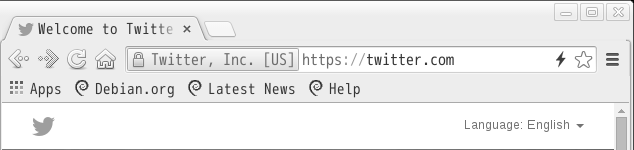
\includegraphics[width=0.9\hsize]{image201507/chromium-http-2-ready_mono.png}
\end{center}
\caption{chromiumでHTTP/2のサイトにアクセス}
\end{figure}

\subsubsection{iceweasel}

 iceweaselを使う場合は次の通りです。まず、iceweaselと、xul-ext-spdy-indicatorをDebianに導入します。
  
\begin{commandline}
$ sudo apt-get install iceweasel xul-ext-spdy-indicator
\end{commandline}
% $

以上の操作を行ったiceweaselでHTTP/2対応のサイトにアクセスすると、青い稲妻マークがアドレスバーに表示されるようになります。

\begin{figure}[H]
\begin{center}
 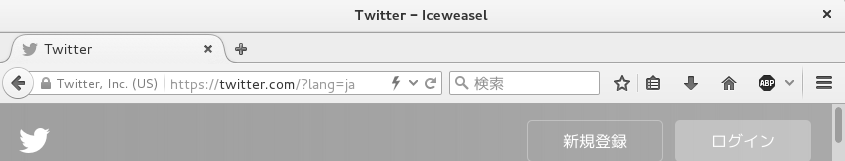
\includegraphics[width=0.9\hsize]{image201507/iceweasel-http-2-ready_mono.png}
\end{center}
\caption{iceweaselでHTTP/2のサイトにアクセス}
\end{figure}

\subsection{サーバ側準備}

 いよいよDebianにサーバ側を準備します。

\subsubsection{HTTP/2に対応しているサーバ}

 どんなサーバがHTTP/2に対応しているかは、\\
\\
 Implementations \\
  \url{https://github.com/http2/http2-spec/wiki/Implementations}\\
\\
 を参照ください。

\subsubsection{nghttp2パッケージ}

 Debian sidにて、HTTP/2対応サーバのパッケージとして、nghttp2があります。ここではこちらを使ってサーバを作ることにします。

 \begin{commandline}
$ sudo apt-get install nghttp2 ssl-cert
\end{commandline}
% $

 なお、閲覧可能なコンテンツとして、groffの付属htmlマニュアルをドキュメントルートにしたHTTP/2サーバを立ててみます。

  なお、*-snakeoil.*というファイルは、ssl-crtパッケージを導入すると勝手に作成される自己証明書ファイルとなります。
  
\begin{commandline}
$ sudo nghttpd -D -d /usr/share/doc/groff-base/html/ \
  443 /etc/ssl/private/ssl-cert-snakeoil.key \
  /etc/ssl/certs/ssl-cert-snakeoil.pem
\end{commandline}  
%$

\subsection{アクセスしてみる}

  ブラウザで、アクセスしてみます。\\
 アクセス先:\url{https://localhost/pic-6.html}

 chromium/iceweasel共に無事にHTTP/2対応を示す青い稲妻マークがURL表示部分に付いていることが判ります。

\begin{minipage}{0.5\hsize}
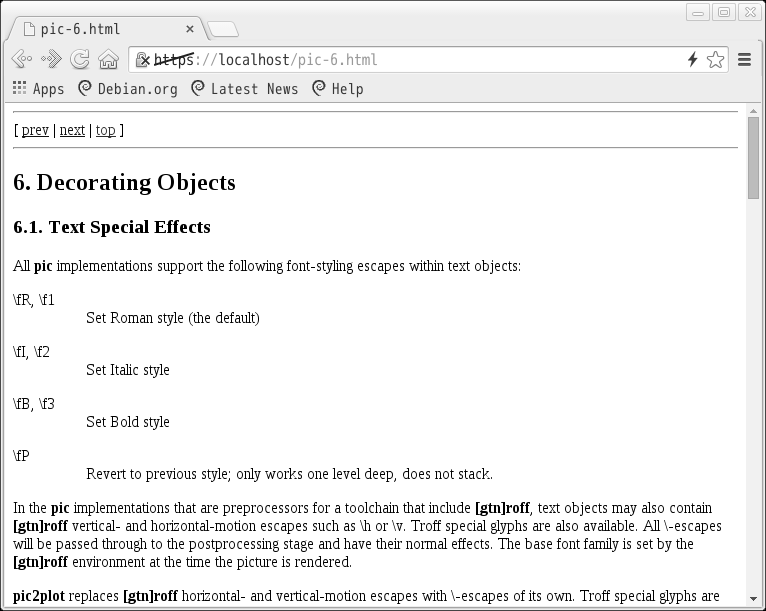
\includegraphics[width=0.9\hsize]{image201507/chromium-groff-access_mono.png}
\end{minipage}
\begin{minipage}{0.5\hsize}
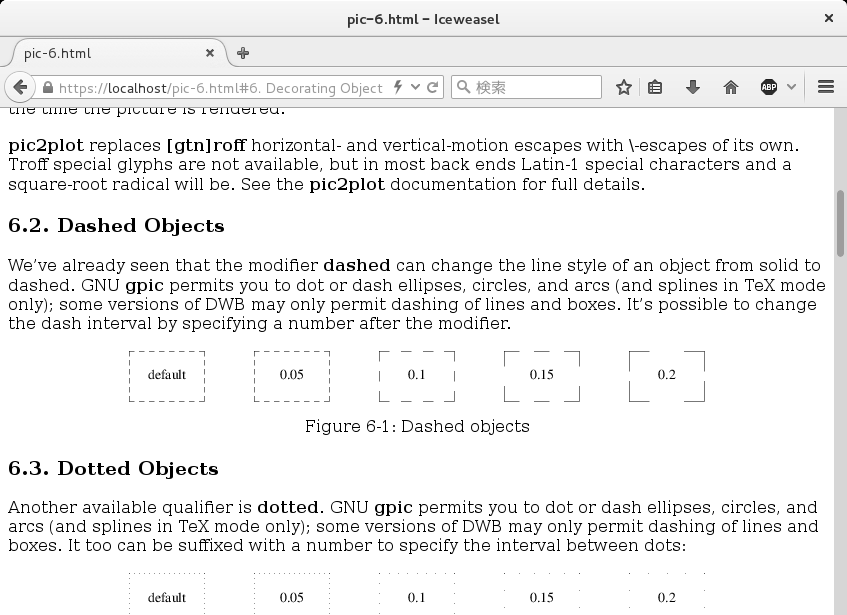
\includegraphics[width=0.9\hsize]{image201507/iceweasel-groff-access_mono.png}
\end{minipage}
 
\subsection{proxyサーバで既存サイトのHTTP/2化をやってみる}

 さて、nghttpdは軽量のHTTP/2対応WEBサーバではあるのですが、やっぱりapacheのような高機能なWEBサーバを使ってHTTP/2を実現したいというニーズがあると思います。(例:phpのサイトをHTTP/2化したい等)

 今度は、apacheをバックエンドにして、nghttp2付属のproxyサーバを使い、サイトのHTTP/2化を行ってみます。
  
 今回用意しようとしている環境の概念図を載せます。

\begin{figure}[H]
\begin{center}
 \includegraphics[width=0.5\hsize]{image201507/nghttpx-apache-proxying-mono.eps}
\end{center}
\caption{proxyサーバでHTTP/2化を行う環境の概念図}
\end{figure}
  
 proxyとapacheの環境をDebianに用意します。手順は次の通りです。

\begin{description}
\item [Step 1.] sudo apt-get install apache2 nghttp2 ssl-cert
\item [Step 2.] sudo a2enmod userdir
\item [Step 3.] cd /home/yours/; mkdir public\_html
\item [Step 4.] cd public\_html; cp -a /usr/share/doc/groff-base/html .
\item [Step 5.] sudo vi /etc/nghttpx/nghttpx.conf\\
\begin{commandline}
 ----nghttpx.confの中身ここから----
frontend=0.0.0.0,443 
backend=127.0.0.1,80 
private-key-file=/etc/ssl/private/ssl-cert-snakeoil.key 
certificate-file=/etc/ssl/certs/ssl-cert-snakeoil.pem 
workers=1 
----ここまで----
\end{commandline}
\item [Step 6.] sudo systemctl start apache2.service
\item [Step 7.] sudo nghttpx -D --conf /etc/nghttpx/nghttpx.conf
\end{description}

 以上できましたら、いよいよ先に用意したブラウザからアクセスしてみます。無事 apache側に用意したサイトが、HTTP/2対応できている事がわかります。\\
\\
 アクセス先:\url{http://localhost/~yours/html/pic.html}\\

\subsection{おわりに}

  HTTP/2もDebianを使えば簡単に実験できます。また、沢山のファイルで構成されるページがあると、HTTP/2は非常に威力を発揮します。この機会にHTTP/2を是非お試し頂き、その威力を確認してみてください。
  
\begin{thebibliography}{9}
\bibitem{ref:http-2-faq} HTTP/2 Frequently Asked Questions,\url{https://http2.github.io/faq/}
\bibitem{ref:server-push-primer} 初めてのHTTP/2サーバプッシュ,\url{http://labs.gree.jp/blog/2014/12/11987/}
\bibitem{ref:wikipedia-http-2} wikipedia HTTP/2の章,\url{https://ja.wikipedia.org/wiki/HTTP/2}
\bibitem{ref:http-2-protocol-upgrade-primer} HTTP/2 プロトコルネゴシエーション方法と ATS での実装,\url{http://techblog.yahoo.co.jp/infrastructure/http2/ats_http2_pn/}
\end{thebibliography}

%201510 tokyo
%-------------------------------------------------------------------------------
\dancersection{NTT フレッツ網経由でNative IPv6}{Roger Shimizu}
%-------------------------------------------------------------------------------
\subsection{はじめに}
NTT フレッツを使っている自宅でIPv6インターネットが動かなかったんです。
\\
NTT NGN 網を使うと、どこかからIPv6 アドレスが割り当てられますし、ゲートウェイも自動的に設定されますが、Internetに繋がらない!
\\
原因は、Dual スタック対応済みDNS が AAAA record (IPv6 address) の結果を、A record と一緒に返します。
\begin{itemize}
\item Google’s DNS: 8.8.8.8 / 8.8.4.4
\item NTT’s DNS: 129.250.35.250 (関東) / 129.250.35.251 (関西)
\end{itemize}
OS側では、IPv6 があれば、IPv4 よりIPv6 が優先的に使われます。
\\
しかし、IPv4へのフォールバックが発生してネットアクセスが非常に遅くなってしまう。
\\
NTT ではそういう状況が把握されているようです、その解決方法はなんと「IPv6 を無効」\footnote{\url{https://flets.com/customer/ipv6_display.html}}となります!
\\
\subsection{DebianではどうやってIPv6 を無効にするの?}
kmod 設定ファイル(squeezeまで使用可能): /etc/modprobe.d/aliases
\begin{commandline}
alias net-pf-10 off
\end{commandline}
sysctl 設定ファイル(動的に変更可能): /etc/sysctl.conf
\begin{commandline}
net/ipv6/conf/all/disable_ipv6 = 1
\end{commandline}
起動時の kernel パラメータ(最初から無効になる): 
\begin{commandline}
ipv6.disable=1
\end{commandline}
/etc/default/grub の GRUB\_CMDLINE\_LINUX 変数に追加が必要です。
Debian Installer なら、起動時に\verb|<TAB>| をしてから上記のパラメータを入力できます。
\\
\subsection{IPv6 体験のための トンネル方式の使い方}
Native 環境が見つからなければ、トンネル方式でなど色々体験する方法があります。
\begin{itemize}
		\item 6in4 (proto-41) (例、{\tt Hurricane Electric さんの tunnelbroker サービス}\footnote{\url{https://www.tunnelbroker.com}})
\item Teredo (例、Debian で miredo というパッケージをインストールすればすぐに使えます)
\item SixXS
\item AICCU
\item AYIYA
\item 6to4 (via 192.88.99.1)
\item 6over4 (fe80:: \& IPv4)
\item freenet6
\end{itemize}
体験・検証ぐらいならそれで良いけど、従来 IPv4 の性能と比べて遅くて、通常に IP トンネルを使用することはおすすめしないと考えております。
\subsection{Tunnel で遅くなる原因の解析}
普通にウェブアクセスが Tunnel 経由なら遅くなる原因は DNS + CDN となります:
\begin{itemize}
\item DNS のレスポンス時間
\item CDN のアクセス時間
\end{itemize}
DNS はどこを使うべきか?例として、アメリカ西海岸の tunnelbroker.net を使うなら、ケース別で解析して見ましょう。
\begin{itemize}
\item Local DNS
\\プロバイダー(ISP) から提供される DNS となり、IPv4 で CDN が日本のサーバに直接アクセス出来て、特に問題がないけれど、
IPv6 だと Host $\rightarrow$ US Tunnel $\rightarrow$ JP CDN にしてしまい、往復で 250ms 位になります。
\item Remote DNS
\\トンネル経由で US 側の DNS となり、毎回 DNS query のコストが 120ms 位になりますし、IPv4/IPv6 両方ウェブアクセス時間も 120ms を加算されるとなってしまいます。
\end{itemize}
どっち側の DNS を使っても、遅くなることが分かりました。
\subsection{NTT フレッツで Native IPv6 ができます!}
Native IPv6 のメリットというと、Local DNS を使うことで、DNS Query コストがあまり掛からないし、IPv4/IPv6 両方共にローカル(又は近くに) CDN が使えます。
多くプロバイダーは IPv6 が対応するようになりました。
\begin{itemize}
\item OCN: \url{http://service.ocn.ne.jp/ipv6/access/}
\item Plala: \url{http://www.plala.or.jp/ipv6/service/area/}
\item So-net: \url{http://www.so-net.ne.jp/common/IPv6/}
\item 他のISP: \url{http://www.jaipa.or.jp/ipv6/}
\end{itemize}
すべては確認していませんが、主な OCN/So-net/Plala などは既に Native IPv6 が対応されているようです。それから、簡単に Dual Stack が構築出来ます!
\subsection{具体的な IPv6 の設定方法}
Dual Stack なら、2本PPPセッションが必要。例えば、
\begin{itemize}
\item ppp0: IPv4
\item ppp1: IPv6
\end{itemize}
IPv4 の PPPoE 設定は従来通りで良くて、IPv6 の方は IPv4 の設定をベースにして、以下の変更が必要となります。
\begin{itemize}
\item cp /etc/ppp/peers/dsl /etc/ppp/peers/dslv6
\item echo +ipv6 \verb|>>| /etc/ppp/peers/dslv6
\item /etc/ppp/peers/dslv6 に、元IPv4のアカウントをIPv6 版に書き換える
\item /etc/ppp/chap-secrets に、IPv6 アカウントのパスワードを追加します(IDは IPv4 / IPv6 別ですが、パスワードは一緒になるケースがほとんどです)
\end{itemize}
IPv6 PPPoE アカウント(CHAP ID)については、プロバイダーによります。
\\例としては、(太字は IPv4 の設定に加えた部分です)
\begin{itemize}
\item {\tt OCN:}\footnote{\url{http://service.ocn.ne.jp/ipv6/access/flow/}}blah@\texttt{ipv6.}ocn.ne.jp
\item {\tt OCN biz:}\footnote{\url{http://www.ocn.ne.jp/business/ftth/withf/spec.html}}blah@bizf\texttt{6}.ocn.ne.jp 又は blah@bizd\texttt{6}.ocn.ne.jp
\item {\tt Plala:}\footnote{\url{http://www.plala.or.jp/ipv6/access/flow/}}blah@\texttt{v6h.}plala.or.jp 又は blah@\texttt{v6m.}plala.or.jp
\item {\tt So-net:}\footnote{\url{http://www.so-net.ne.jp/option/others/ipv6/}}taro@aa2\texttt{-v6}.so-net.ne.jp
\end{itemize}
また、IPv6 address と default route もそれぞれ設定が必要です。
\begin{itemize}
\item IPv6 address は DHCPv6 クライアント (wide-dhcpv6-clientなど) で取得します。
\item IPv6 default route は手動設定となり、\footnote{\url{https://bugs.debian.org/477245}}\footnote{\url{https://github.com/paulusmack/ppp/issues/40}}
\begin{commandline}
ip -6 r add default dev ppp1
\end{commandline}
で済みます。
\end{itemize}
設定の参考: \url{https://youtu.be/bJ9p2j9frtA}
(git repo: \url{https://github.com/rogers0/config/tree/network/flets-native-v4v6})
\subsection{用語定義}
\begin{itemize}
\item stateless host: IPv6 address と default gateway は RA (ブロードキャスト)による取得します(デフォルト)。
\item stateful host: IPv6 address は DHCPv6 クライアントとして、サーバから取得します。
\item gateway: IPv4 の NAT 機器のような IP パケット転送の機器となります。IPv4 NAT の場合は Address 変換するんですが、IPv6 の場合はルータ機能を加えられます。
\end{itemize}
\subsection{解決案 0: stateful gateway 向け}
デフォルトの stateless host から、stateful host の方式にすると、NTT NGN からの RA (ブロードキャスト) を受けないようになります。
\begin{commandline}
sysctl.conf
	net/ipv6/conf/default/accept_ra = 0
	net/ipv6/conf/all/accept_ra = 0
	net/ipv6/conf/eth0/accept_ra = 0
	net/ipv6/conf/wlan0/accept_ra = 0
\end{commandline}
\subsection{解決案 1: stateless host 向け}
{\tt MSFT の KB}\footnote{\url{https://support.microsoft.com/ja-jp/kb/2551233}}によると解決方法がありました。
それから、他の記事\footnote{\url{http://www.attn.jp/maz/p/i/policy-table/}}も参考にできます。
address selection でNTT NGN 用の prefix の優先度を下げると、問題が解決できます。提示する win32 コマンドを Linux に翻訳すると、
\begin{commandline}
	ip addrlabel add prefix 2001:c90::/32   label 8
	ip addrlabel add prefix 2404:1a8::/32   label 8
	ip addrlabel add prefix 2408::/22           label 8
	ip addrlabel add prefix 2001:d70::/30   label 8
	ip addrlabel add prefix 2001:a000::/21 label 8
\end{commandline}
となります。参考の設定: \url{https://github.com/rogers0/config/tree/network/stateful_v6host}
\subsection{ゴールまで足りないもの (TODO)}
\begin{itemize}
\item Firewall: ip6tables
\item stateful IPv6 gateway (allow IPv6 forward)
\item stateful/stateless IPv6 host (disallow IPv6 forward)
\end{itemize}

%kansai201508
\dancersection{wiki:Subkeys}{かわだてつたろう}

{\tt Debian Wiki}\footnote{\url{https://wiki.debian.org/}}には{\tt Debian}に関す
る様々な情報がまとめられています。そのなかで{\tt OpenPGP}のサブキー(副鍵)に関する
ページ{\tt wiki:Subkeys}\footnote{\url{https://wiki.debian.org/Subkeys}}
がありましたので、その内容を紹介します。

\subsection{鍵とは}

{\tt OpenPGP}は公開鍵暗号方式で秘密鍵と公開鍵の2つの鍵から成り立つ暗号方式です。
その名前の通り、公開鍵は公開するための鍵、秘密鍵は自分だけが使う鍵です。秘密鍵
は署名や公開鍵で暗号化されたメッセージの復号化に使用します。

\subsection{副鍵とは}

鍵を作成時に必ず作成される鍵ペアが主鍵(マスターキー)です。この他に作成する鍵ペア
を副鍵と呼びます。副鍵は署名、暗号化など通常の鍵として使用でき、主鍵とは別に破棄
することもできます。つまり、主鍵と結び付いている独立した鍵ペアといえます。

\subsubsection{GnuPGでの副鍵}

{\tt GnuPG}では、主鍵は署名にしか使用できません。暗号化するためには副鍵を作成する
必要があります。

鍵作成時の次の選択で(署名のみ)を選択していなければ副鍵が作成されているはずです。

\begin{commandline}
Please select what kind of key you want:
   (1) RSA and RSA (default)
   (2) DSA and Elgamal
   (3) DSA (sign only)
   (4) RSA (sign only)
Your selection?
\end{commandline}

このようになっているのは{\tt RSA}が特許の関係で使用できなかったころ、
{\tt ElGamal}は暗号化のみ、{\tt DSA}は署名のみにしか使用できないといった歴史的理
由もあるようです。


\subsection{なぜ副鍵}

主鍵は非常に大事です。主鍵の秘密鍵が失なわれるとあなたの信用も失なわれ、信頼の輪
をまた一から築きあげることになります。そのため、主鍵の秘密鍵は非常に非常に安全に
保管しておく必要があります。しかし、安全にすればするほど日常の使用は不便なものに
なります。

これを解決するのに副鍵を使います。暗号化用の副鍵と同じように署名用の副鍵を作成し
公開すれば、副鍵で署名して使うように副鍵で署名して使うことができます。

次のような鍵の変更は主鍵でしかできません。

\begin{itemize}
\item 他の人の鍵に署名を追加するか、既存の署名を取り消す
\item 新しい{\tt UID}を追加するか、{\tt UID}に{\tt primary}マークを付ける
\item 新しい副鍵を作る
\item 既存の{\tt UID}または副鍵を失効する
\item {\tt UID}の{\tt preferences}を変更する(例: {\tt setpref})
\item 主鍵または副鍵の期限日を変更する
\item 鍵の失効もしくは失効証明書の生成
\end{itemize}

{\tt Web of Trust}のリンクは公開鍵と{\tt UID}の組合せに対する署名です。
{\tt OpenPGP}では主鍵の秘密鍵から{\tt UID}への署名のリンクで副鍵は関係がありませ
ん。主鍵が安全であれば副鍵だけ盗まれても副鍵だけ失効し再作成することで済みます。


\subsection{どのようにするか}

次の手順をとります。

\begin{enumerate}
\item 念のため既存の{\tt GnuPG}ファイルのバックアップをとる
  \begin{commandline}
$ umask 077; tar -cf $HOME/gnupg-backup.tar -C $HOME .gnupg
  \end{commandline}
\item 署名用の副鍵を作る
  \begin{commandline}
$ gpg --edit-key YOURMASTERKEYID
gpg> addkey
Key is protected.

You need a passphrase to unlock the secret key for
user: "WHO <who@example.org>"
2048-bit RSA key, ID AAAAAAAA, created 2015-01-01

Enter passphrase: YOURMASTERKEYPASSWORD

Please select what kind of key you want:
   (3) DSA (sign only)
   (4) RSA (sign only)
   (5) Elgamal (encrypt only)
   (6) RSA (encrypt only)
Your selection? 4

RSA keys may be between 1024 and 4096 bits long.
What keysize do you want? (2048)

Requested keysize is 2048 bits
Please specify how long the key should be valid.
         0 = key does not expire
      <n>  = key expires in n days
      <n>w = key expires in n weeks
      <n>m = key expires in n months
      <n>y = key expires in n years
Key is valid for? (0)

Key does not expire at all
Is this correct? (y/N) y
Really create? (y/N) y

gpg> save
  \end{commandline}
\item {\tt \$HOME/.gnupg}をUSBドライブにコピーするなどして退避させる
\item 主鍵の秘密鍵を取り除いた状態にする
  {\tt GnuPG}にそのためのコマンドがないので次の手順を踏む
  \begin{enumerate}
  \item 副鍵の秘密鍵をエクスポート
    \begin{commandline}
$ gpg --export-secret-subkeys YOURMASTERKEYID > secret-subkeys
    \end{commandline}
  \item 主鍵と副鍵の秘密鍵を削除
    \begin{commandline}
$ gpg --delete-secret-key YOURMASTERKEYID
    \end{commandline}
  \item 副鍵の秘密鍵を戻す
    \begin{commandline}
$ gpg --import secret-subkeys
    \end{commandline}
  \item {\tt sec}が{\tt sec\#}と表示されており、主鍵の秘密鍵が取り除かれているこ
    とを確認する
    \begin{commandline}
$ gpg -K
------------------------
sec#  2048R/AAAAAAAA 2015-01-01
uid                  WHO <who@example.org>
ssb   2048R/BBBBBBBB 2015-01-01
ssb   2048R/CCCCCCCC 2015-01-01
    \end{commandline}
  \end{enumerate}
\item 鍵のパスワードを変更する
  \begin{commandline}
$ gpg --edit-key YOURMASTERKEYID passwd
  \end{commandline}
\end{enumerate}

これで準備が整いました。後は通常通り使用するだけです。

\subsubsection{主鍵が必要な場合は}
環境変数{\tt GNUPGHOME}か{\tt --homedir}オプションで退避させた{\tt .gnupg}ディレ
クトリを指定して使用します。

\begin{commandline}
$ export GNUPGHOME=/path/to/save/.gnupg
$ gpg -K
\end{commandline}

\begin{commandline}
$ gpg --homedir=/path/to/save/.gnupg -K
\end{commandline}

\subsubsection{cross-certification}

署名用の副鍵は主鍵と{\tt cross-certification}(相互署名)しておくことがすすめられ
ています。

主鍵と副鍵が同一のIDに属していることを保障するために、主鍵と副鍵の鍵束は主鍵によっ
て署名されます。これで鍵束が主鍵に属していることがわかりますが、副鍵から見た場合、
本当にこの副鍵が主鍵の持ち主のものかがわかりません。他人が副鍵を入手して主鍵で鍵
束に署名した状態と区別がつかないためです。そのため、副鍵でも鍵束に署名するのが相
互署名です。

{\tt GnuPG}で相互署名するには次のコマンドを実行します。

\begin{commandline}
$ gpg --edit-key YOURMASTERKEYID
gpg> cross-certify
\end{commandline}

相互署名してない場合、{\tt GnuPG}が次の警告を出します。

\begin{commandline}
gpg: WARNING: signing subkey CCCCCCCC is not cross-certified
gpg: please see http://www.gnupg.org/faq/subkey-cross-certify.html for more information
gpg: Can't check signature: general error
\end{commandline}

次のところを参考にしてください。
\begin{itemize}
\item {\tt Signing Subkey Cross-Certification --- GnuPG.org}\footnote{\url{https://www.gnupg.org/faq/subkey-cross-certify.html}}
\item {\tt [mew-dist 28255] Re: gnupg 1.4.9}\footnote{\url{http://www.mew.org/ml-archives/mew-dist/2008-April/027942.html}}
\end{itemize}

\subsection{それから何する}

キーリング、キーサーバーへ登録します。

\begin{commandline}
$ gpg --send-key YOURMASTERKEYID
\end{commandline}


\subsection{まとめ}

手順が少し手間ですが、主鍵を日常の使用と切り離せるのは安心感があります。

とはいえ、主鍵を安全にしておかないといけないことに変わりはありません。
そのためには{\tt Gnuk Token}\footnote{\url{http://www.fsij.org/category/gnuk.html}}
などを使うのがよいかもしれません。

%201510 tokyo
%-------------------------------------------------------------------------------
\dancersection{DebConf15 ビデオ紹介}{野島 貴英}
%-------------------------------------------------------------------------------

\subsection{はじめに}

 毎年1回、世界中のDebian Project関係者及び熱心なユーザらが集まり、ハッカソンをしたり、発表をしたりするイベントとして、DebConfがあります。16回目\footnote{DebConf 0があるため}の開催のDebConf15が、2015/8/15-22の間、ドイツのハイデルベルクで開かれました。

 公式URLは \url{http://debconf15.debconf.org/}となります。

 ここでは、Debconf15で行われたセッションのうち、字幕ファイルが用意されているものについて紹介してみます。

\subsection{DebConf15 セッションのビデオ}

 DebConfでは、Video Teamが各セッションをビデオに撮り公開しているため、いつでもセッションの内容を見ることができます。なお、Debianはフリー(自由)にこだわるため、フリーなフォーマットである、webmが動画フォーマットとして利用されています。

 掲載先:\url{http://debconf15.debconf.org/videostream.xhtml}

 しかしながら、iphone/Androidのスマートフォンで気軽に見たいという今時のニーズもあるかと思います。幸い、youtubeでもDebConf15のビデオが公開されていましたので紹介しておきます。

 youtube:\url{https://www.youtube.com/playlist?list=PLz8ZG1e9MPlz2bUTzfgJhOJCxwT866D4w}
  
\subsection{DebConf15 ビデオ字幕編}

 DebConfは世界中からDebian Project関係者、及び、ユーザが集まるイベントですので、公用語は全て英語になります。発表も英語です。英語を母国語としない人にとってはヒアリングが苦手な方もいらっしゃいます。こういった人のために、現状、数は少ないですが、いくつかの英語の字幕が起こされています。

 字幕取得先:\url{http://ftp.acc.umu.se/pub/debian-meetings/2015/debconf15/subtitles/english/}

 字幕ファイルの使い方は次の通りです。
 
  \begin{description}
\item [Step 1.] 先のURLから、*.srtファイルを取得する。
\item [Step 2.] totem/vlc/mplayerなどでDebConf15の動画を開き、字幕というメニューを選んで対応する.srtファイルを指定します。ファイル名はセッションの名前になっています。
  \end{description}    
  
 字幕付き再生をDebian sid上で行っている様子を載せます。
  
\begin{figure}[H]
\begin{center}
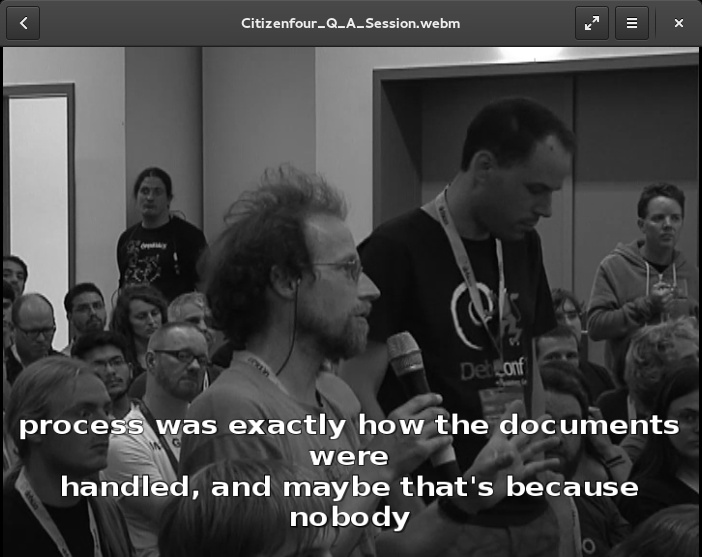
\includegraphics[width=0.5\hsize]{image201510/subtitle_mono.png}
\end{center}
\caption{字幕付き再生例}
\end{figure}

\subsection{今回のビデオ紹介}

 今回紹介予定の具体的なセッション名は、

\begin{itemize}
\item Stretching out for trustworthy reproducible builds
\item Thanks for maintaining a desktop environment. But is it accessible?
\end{itemize}

となります。

\subsection{Stretching out for trustworthy reproducible builds}

 ドイツの有名なChaos Computer Club\footnote{Wikipedia-jpで引いてみて下さい。ドイツの有名なコンピュータ技術のエキスパート集団。}にも所属されているDebian開発者らによる、Reproducible Buildsについてのセッションです。

\begin{figure}[H]
\begin{center}
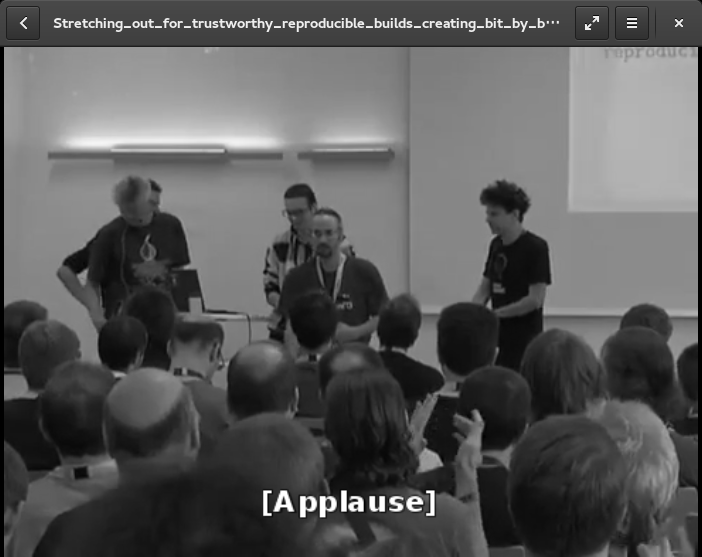
\includegraphics[width=0.5\hsize]{image201510/reproduct_mono.png}
\end{center}
\caption{Stretching out for trustworthy(略)の発表}
\end{figure}

如何にビデオの内容をかいつまんで紹介します。

\subsubsection{動機}

 \begin{itemize}
 \item The 31st Chaos Communication Congress (31C3)\footnote{Chaos Computer Club主催の毎年行われるイベント}にて、パッケージのバイナリにトロイの木馬が巧妙に仕掛けられているか?を調べるにはReproducible Buildsをしたほうが良いという発表を行ったとのことです。
\item 31C3のわずか数カ月後に今度はEdward Snowdenさんにより、CIAのStrawhourseというコード名に関するCIA conference 2012の内部文章がリークされました。内容は、MacOS/iOSのSDKに不当な改造を行い、生成されるバイナリにCIAが利用するためのトロイの木馬を仕掛けるという驚くべき内容でした。これにより、Reproducible Buildsが益々急務になったとのことです。なお、リーク文章は、\url{https://theintercept.com/document/2015/03/10/strawhorse-attacking-macos-ios-software-development-kit/}で参照できます。
 \end{itemize}

\subsubsection{セキュリティ以外の良い点}

\begin{itemize}
 \item ビルド環境によらず同じバイナリができる、また、クロスビルドの確認ができるようになる、
 \item Debug packageがいつでも(バイナリ作ったあとでも)作れるとか、
 \item FTBFS\footnote{Fails To Build From Sourceの略}が早くわかるとか、
 \item バージョン上げた時の.debの差分が小さくなるとのことです。
 \end{itemize}

\subsubsection{現在のReproducible Builds状況は次の通り}

 \begin{itemize}
 \item Bitcoin/Tor/Corebootは完了している。
 \item Debian/FreeBSD/NetBSD/OpenWrtは進行中。
 \end{itemize}

\subsubsection{工夫と苦労}
 
\begin{itemize}
\item 環境変数SOURCE\_DATE\_EPOCHに時刻(エポック秒)を指定すると、その時刻でビルドしたようにビルドするように様々なツールを改造しupstreamへ提供し取り込んでもらったそうです。なお、これだけでは足らないパッケージが沢山あったらしく、ビルドの日付が埋め込まれる部分をReproducible Builds出来ないとBTSしたりして対策も多数したとのことです。
\item tarにビルド環境の都度のユーザ名、グループ名が混じってしまう件を対策したそうです。
\item ファイルシステムとlocale環境変数(LANG,LC\_ALL変数)との違いによるソートの振る舞いの違い、プログラムの出力が異なってしまう件の対策をしたそうです。
\end{itemize}

言われてみると「なるほど!」と気がつく事ばかりで、考えてみれば相当に苦労するような内容ばかりでした。

\subsubsection{視聴後の所感}

よく、巷では簡単にReproducible Buildsは、パッケージのセキュリティ確認の為と簡単に紹介されますが、実はDebianを構成する重要なソフトウェア・パッケージの多くに手を加えなければ実現できないという大変な偉業を果たしていたという内容でした。思わず、これらの偉業に拍手をしたくなりました。

\subsection{Thanks for maintaining a desktop environment. But is it accessible?}

 Debian ProjectにてAccessibilityを担当されている方の発表となります。
Accessibilityに関しての現状と苦労がわかる発表内容となっています。

 プレゼン資料は:\url{http://brl.thefreecat.org/2015-08-22-debconf.pdf}

\begin{figure}[H]
\begin{center}
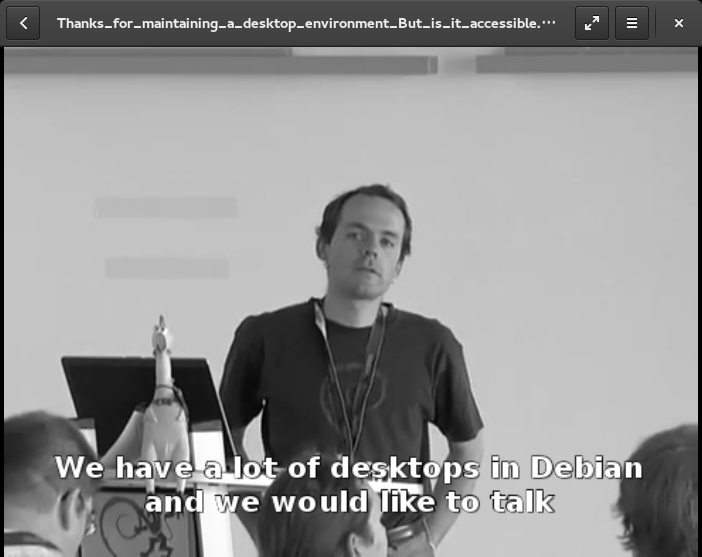
\includegraphics[width=0.5\hsize]{image201510/accessibility_mono.png}
\end{center}
\caption{Thanks for maintaining a desktop...(略)の発表}
\end{figure}

\subsubsection{Accessibilityについてうっかりすると忘れがちになる大変重要な事}

 Free Softwareは、問題があったり、気に入らなかったら、自分で直せるということが基本であるが、Accessibilityの機能を必要としている人は、基本的に治したくても直せない場合が多いので、コミュニティーによる修正・改善が必須です。

\subsubsection{Linux Desktop環境のAccessibilityの現状}

\begin{itemize}
  \item Linuxで動作するDesktop環境は、GNOMEがAccessibilityが最もよくできている状況です。
  \item しかしながら、GNOME3を持ってしても、Windowsに比べると10年単位で遅れており、Appleの製品に比べると石器時代の代物と言われても仕方が無い状況です。
  \item 弱視の人には、合成音声によるサポートは厳しい場合(そもそも発音しにくいワードの場合など)があるため、理想的には、Piezo braille cellをサポートすべきです。
\end{itemize}

\subsubsection{Linux Desktop環境のAccessibilityの現状の仕組みと開発方法}

先のプレゼン資料、及び、ビデオにて

\begin{itemize}
  \item LinuxのAccessibilityのフレームワーク、
  \item LinuxのAccessibilityのテスト環境など
 \end{itemize}

が紹介されています。先述のプレゼン資料を参照ください。Accessibilityがどのようにできていて、どうテストすべきかについて、非常に良い資料となっています。

\subsection{おわりに}

 紙面の関係で今回はセッションを2つのみ紹介しましたが、他にも非常に興味深いセッションがあります。なにぶん英語のセッションなので、見て理解するのに苦労する状況ですが、その努力を払っただけの収穫があるのが、Debconfのビデオです。是非、1つ見て、内容を考えてみませんか?きっと、今まで見えていた世界ががらっと変わるような体験が出来ると思っています。

%201511 kansai KOF
\dancersection{Debian と arm64サポート}{岩松 信洋}

  \subsection{arm64}
  \begin{itemize}
  \item Debian 8.0 から arm64 サポートが入った
  \item Debian でサポートする ARM アーキテクチャ
 \begin{itemize}
  \item armel\\
  32bit / litte endian / ARMv5t

  古いNAS(QNAP、Buffalo、etc)やルータで使用されている ARM SoCで利用可能。

  \item armhf\\
  32bit / litte endian / ARMv7 + VFP3(浮動小数点演算ユニット)

  Raspberry Pi \textcolor{black}{2} などで利用可能。

  \item arm64 $\leftarrow$ \textcolor{black}{New!}

  \end{itemize}

  \item Raspbian

  \begin{itemize}
  \item 32bit / litte endian / ARMv6 + VFP2(浮動小数点演算ユニット)

       Raspberry Pi \textcolor{black}{1} などで利用可能。
  \item Raspbian in not Debian

  \end{itemize}

  \end{itemize}

  \begin{itemize}
  \item ARMv8 (ARM Version 8)
  \end{itemize}
  \begin{center}
  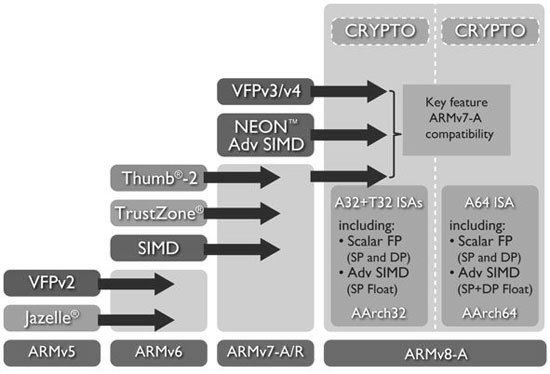
\includegraphics[width=0.7\hsize]{image201511/V5_to_V8_Architecture_mono.jpg}
  \end{center}

\begin{minipage}{0.7\hsize}
\begin{itemize}
\item ARMv8 (ARM Version 8)
\item オリジナルコアとしてはCortex-A57、ARM Cortex-A53とCortex-A72がある
\item 正式名称はAArch64
\item Linux kernel では わかりにくいということで arm64 に\\
\url{https://lkml.org/lkml/2012/7/15/133}
\item Debian もこれに追従して arm64 とした
\item コンパイラなどのトリプレットは aarch64-linux-gnu 
\item GCC の定義は \_\_aarch64\_\_ 
\item 紛らわしいので注意
\end{itemize}
\end{minipage}
\begin{minipage}{0.25\hsize}
%コピーライト未確認のため
%
\includegraphics[width=0.8\hsize]{image201511/1254383-arm-aarch-64-300x250.jpg}
\end{minipage}

  \subsection{Debian ARM 開発体制}

  \begin{itemize}
  \item 2012 年から開発開始
  \item 開発に参加している多くのDebian Developer が Linaro 所属

   Steve McIntyre、 Wookey、Riku Voipio など

  \item GCC/binutils:Matthias Klose (GCC Upstream, Ubuntu Developer でもある)
  \item libc:Aurelien Jarno、libc メンテナチーム
  \item Linux kernel:Ben Hutchings(Linux 3.2 LTS メンテナ)、Ian Campbell(Xen、Allwinner SoCs 関
連)、その他大勢

  % \item Linaro の成果が Debian と Ubuntuに回るサイクルができている

  \end{itemize}

  \subsection{Debian ARM 開発体制}

  \begin{itemize}
  \item Buildd: Applied Micro の X-gene を使ったサーバで運用中
     \url{https://buildd.debian.org/status/architecture.php?a=arm64&suite=sid}
  \item SoC: X-C1 / 2.4Ghz / 8コア 独自コア

  \begin{center}
  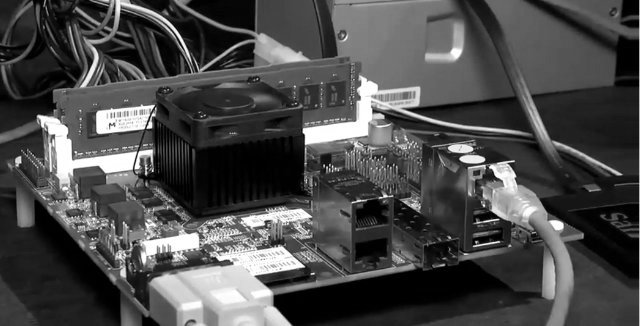
\includegraphics[width=0.7\hsize]{image201511/x-gene_mono.jpg}
  \end{center}

  \end{itemize}



%FIXME not find image201511/graph-week-big.png
%
%  \subsection{Debian ARM 開発体制}
%
%  \begin{center}
%  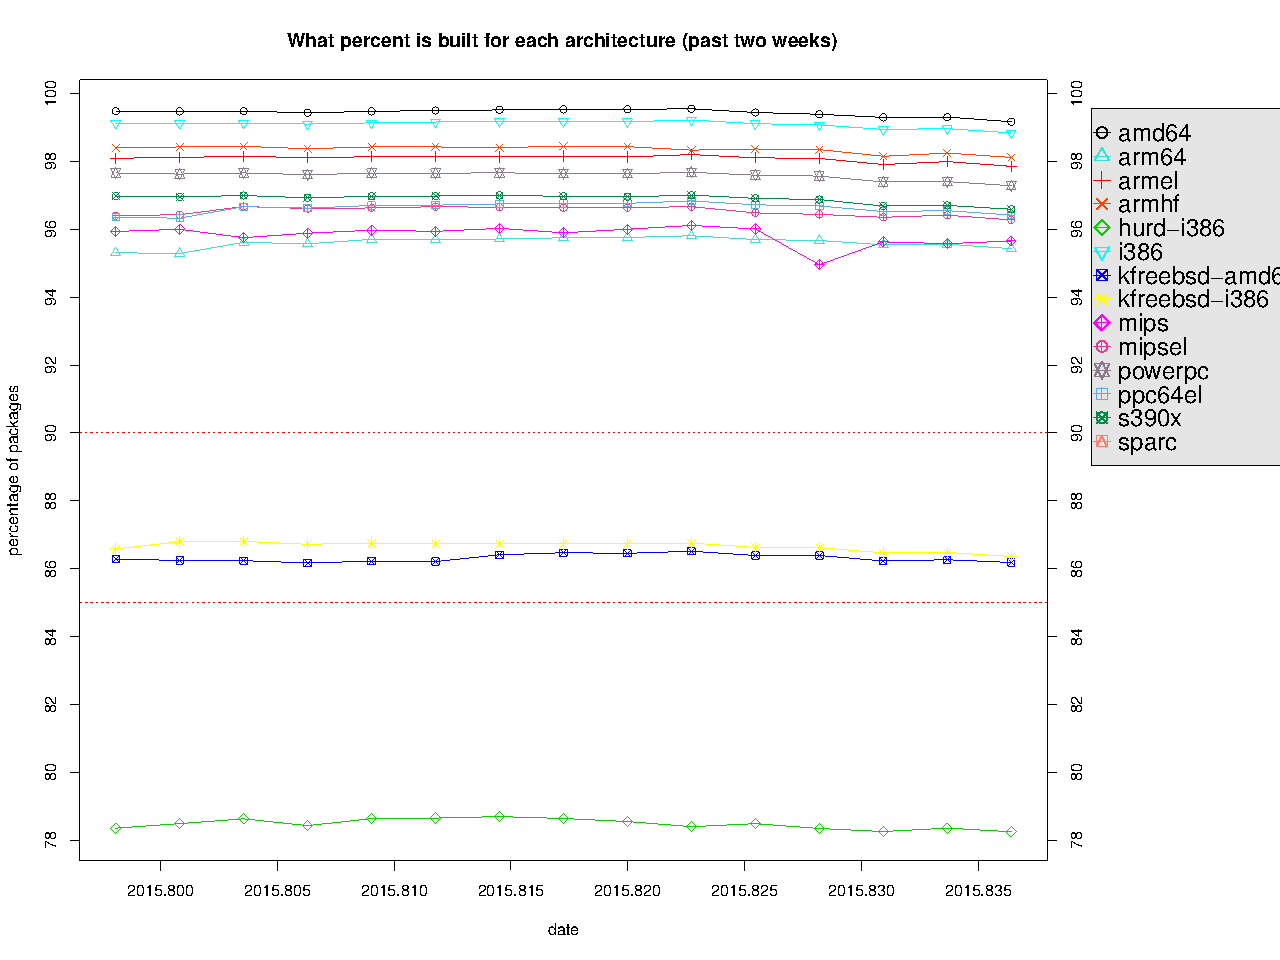
\includegraphics[width=0.7\hsize]{image201511/graph-week-big.png}
%  \end{center}
%
%



  \subsection{クロスコンパイル環境}
  \begin{itemize}
  \item Jessie リリース後Debianのクロスコンパイル環境が変わった
  \item 今まではEmdebianから提供されているパッケージを使うか、ユーザ自身でパッケ
ージ化する必要があった。$\leftarrow$ 手間がかかる。

  \item GCCメンテナによりクロスコンパイル用パッケージが提供されるように

  \begin{itemize}
    \item クロス用binutils $\rightarrow$ binutils ソースパッケージ
    \item クロス用libc $\rightarrow$ cross-toolchain-base ソースパッケージ
    \item クロス用GCC $\rightarrow$ gcc-5-cross ソースパッケージ

\begin{commandline}
    $ sudo apt-get install gcc-5-aarch64-linux-gnu
\end{commandline}

  \end{itemize}

  \item リリース対象外のアーキテクチャは未サポート
  \end{itemize}



  \subsection{ユーザランドイメージ}
  \begin{itemize}
  \item インストーラが用意されている \\
	  \url{https://www.debian.org/CD/http-ftp/#stable}
  \item cdebootstrap を使うのが簡単

\begin{commandline}
   $ sudo cdebootstrap --foreign --arch arm64 \
         jessie /tmp/root http://http.debian.net/debian/
\end{commandline}
  \end{itemize}




  \subsection{サポートボード}
  \begin{itemize}
  \item Debian では ARM リファレンスボード(Juno)と X-gene(Applied Micro)のみサポート。
  \item arm64 のボードは値段が高い(10万円以上)上に入手性が悪い。
%FIXME not find image201511/juno.jpg 
%  \begin{center}
%    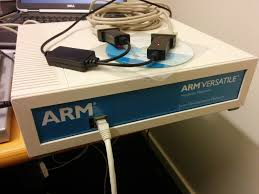
\includegraphics[width=0.5\hsize]{image201511/juno.jpg}
%  \end{center}
  
  \end{itemize}

  \begin{itemize}
    \item 96boards (Linaro Community Board Program) から入手するのがよさげ。約1万円。
    \begin{center}
    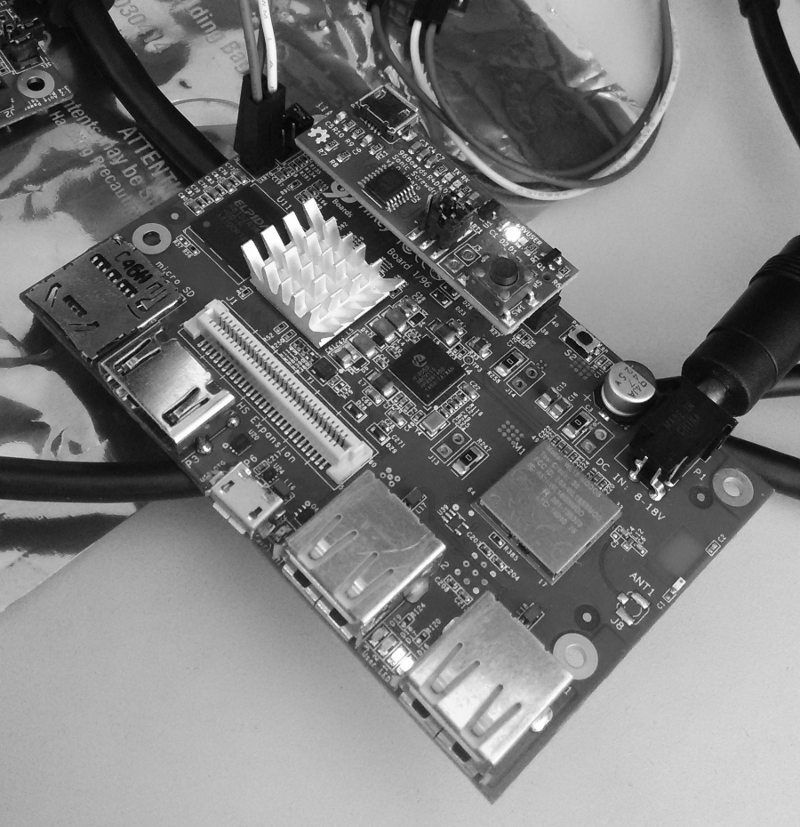
\includegraphics[width=0.3\hsize]{image201511/hikey_mono.png}
    \end{center}
    \begin{itemize}
    \item Linux カーネルパッケージが更新され次第、Debian でもサポートする予定。
    \end{itemize}
  \item QEMU を使って開発することも可能。ただし QEMU 2.0以降。
  \end{itemize}



  \subsection{ベンチマーク}

\begin{table}[htb]
  \begin{tabular}{|l|l|l||l|} \hline
    ベンチマーク  & Raspberry Pi 2 & ODROID-XU4 & Hikey  \\ \hline \hline
    Dhrystone-2 & 1006.6 & 3994.1 & \textcolor{black}{2943.7} \\ \hline
    Double-Precision Whetstone & 361.0 & 1024.9 & \textcolor{black}{680.3} \\ \hline
    Nbench 2.2.3 Integer  & 20.419 & 61.227  & \textcolor{black}{30.803} \\ \hline
    Nbench 2.2.3 FP  & 8.434 & 25.369 & \textcolor{black}{11.889} \\ \hline
  \end{tabular}
\end{table}

\begin{itemize}
\item Raspberry Pi 2: Broadcom BCM2836 900MHz  ARM Cortex-A7 4 core
\item ODROID-XU4: Samsung Exynos5422 Cortex-A15 2Ghz and Cortex-A7 Octa core CPUs
\item Hikey: HiSilicon Kirin 6220 Cortex-A53 1.2Ghz Octa core
\end{itemize}

 \begin{center}
 \textcolor{red}{\texttt{ODROID-XU4 > Hikey > Raspberry Pi 2}}
 \end{center}



%
%  \subsection{ベンチマーク}
%  \begin{center}
%  \includegraphics[width=0.3\hsize]{image201511/20110809aa_20110809185955.jpg}
%  \end{center}
%


  \begin{itemize}
  \item いまのところ ARMv7 の方が速い。
  \item Cortex が遅いという話も。独自コアのSoCはそこそこ速い。
  \item といってもこのまま32bit ARM を使っても2038年問題が。
  \item Cortex-A72 に期待。
  \end{itemize}



  \subsection{まとめ}
  \begin{itemize}
  \item Debian では ARM64 が既に使える環境が整っている。
  \item Upstream や 周辺組織との連携も十分。
  \item クロスコンパイル環境もオフィシャルでサポートされるようになり、今まで以上に開発しやすくなっている。
  \item ボードの供給問題がネック。一般向けは 96boards 頼り。
  \item 上記の理由もあり、サポートボードは少ない。今後頑張って増やします。
  \end{itemize}


%201509tokyo
\dancersection{Debian パッケージング道場 git buildpackageの使い方}{岩松 信洋}

Debian パッケージングチュートリアル\footnote{https://www.debian.org/doc/manuals/packaging-tutorial/packaging-tutorial.ja.pdf}であまり解説されていない gbp (git
buildpackage) の基本的な使い方について説明する。

\subsection{VCS で管理しない場合}

\begin{center}
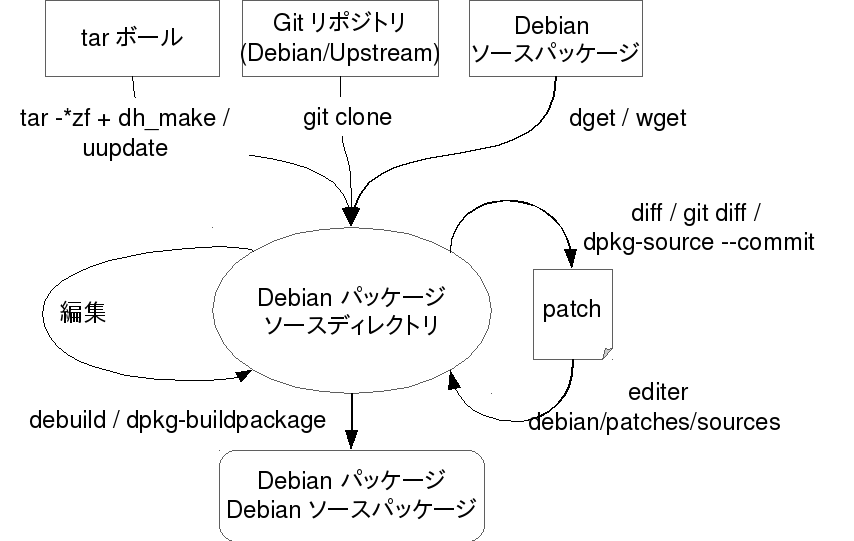
\includegraphics[width=0.8\hsize]{image201509/gbp-images0_mono.png}
\end{center}


\subsection{VCS で管理する場合}
\begin{center}
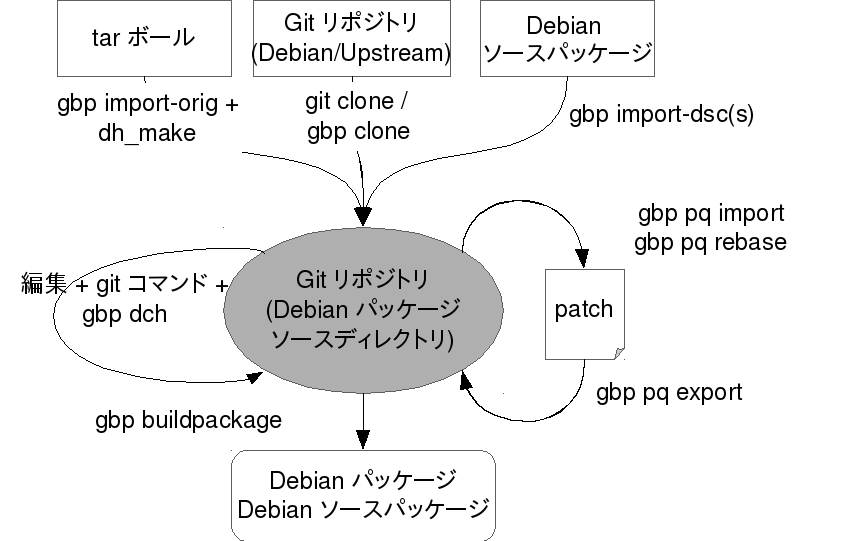
\includegraphics[width=0.8\hsize]{image201509/gbp-images1_mono.png}
\end{center}

\subsection{Upstream から tar ボールがリリースされている場合}

Upstream からtarボールがリリースされている場合、
tar ボールをGitリポジトリにコミットした後、パッケージ化を行う。


\begin{itemize}
\item tar ボールをダウンロードする

\begin{commandline}
$ wget package-name-0.0.1.tar.gz
\end{commandline}

\item Gitリポジトリを作成する

\begin{commandline}
$ git init package-name
$ cd package-name
\end{commandline}

必要であれば git config で Git の設定を変更する。
\end{itemize}

\begin{itemize}
\item tar ボールを指定して、ソースコードを Git にコミットする

\begin{commandline}
$ gbp import-orig --pristine-tar \
	../package-name-0.0.1.tar.gz
$ git tag 
$ upstream/0.0.1
$ git branch
* master
  upstream
\end{commandline}
\end{itemize}

\begin{itemize}
\item Upstreamのコードは upstream ブランチで管理され、同時にタグが設
定される。
\item pristine-tar オプションはオリジナルのtarボールの差分を保存するための仕組みを有効
にする。Upstreamのコードは upstream ブランチで管理され、Debian パッケージを
作成するときに、そこから orig.tar.gz ファイルを作成する。この時に作成されるファイル
が同じものにならない場合がある。Debian では
取り込んだ tat.gz ファイルのハッシュ値とDebian ソースパッケージとしてアップロードされる
tar.gz ファイルが同じである必要があるため、本オプションを用いて orig.tar.gzとの差分を
バイナリパッチとして保存し、orig.tar.gzを構築する度に再適用することで、ハッシュ値
が同じorig.tar.gzを再構築できるようにしている。
\end{itemize}

\begin{itemize}
\item dh\_make で debian ディレクトリの雛形を作成する 

\begin{commandline}
$ dh_make -p package-name_0.0.1
\end{commandline}

\item debian ディレクトリ内をいろいろ変更する

\begin{commandline}
$ いろいろ修正
$ git add debian
$ git commit
\end{commandline}
\end{itemize}

\begin{itemize}
\item パッケージ化作業ができたら パッケージを構築する

\begin{commandline}
$ gbp buildpackage --git-pristine-tar
\end{commandline}

\item piuparts などでインストール、アンインストールのテスト

\item 最後にクリーンな環境でビルドテスト

\begin{commandline}
$ git-pbuilder
or
$ gbp buildpackage --git-pbuiler --git-pristine-tar
\end{commandline}
\end{itemize}

\begin{itemize}
\item タグを設定して リモートリポジトリにプッシュする

\begin{commandline}
$ gbp buildpackage --git-tag-only
$ git push
\end{commandline}

\end{itemize}

\subsection{upstream に更新があった場合}


\begin{itemize}
\item upstream のtar ボールを取得する

\begin{commandline}
$ wget package-name-0.0.2.tar.gz
\end{commandline}

\item tar ボールを指定してリポジトリにソースコードをコミットする

\begin{commandline}
$ gbp import-orig --pristine-tar \
		../package-name-0.0.2.tar.gz
\end{commandline}

\texttt{--uscan} オプションでダウンロード $\rightarrow$ コミットが一度にできる。
また、ソースコードは自動的にマージされます。マージしたくない場合は
\texttt{--no-merge} を指定して実行する。
\end{itemize}

\begin{itemize}
\item debian/changelog を修正

\begin{commandline}
$ dch -i
or
$ gbp dch 
\end{commandline}

\item パッケージをビルド

\begin{commandline}
$ gbp buildpackage --git-pristine-tar \
		--git-pristine-tar-commit
\end{commandline}

\end{itemize}


% -------------------------------------------------

\subsection{Upstream が Git で管理されている場合}

\begin{itemize}
\item  Upstream では tar ボールでリリースされず、Gitのタグのみでリリースされる場合
もある。
\item Github で開発されているプロジェクトが良い例。
\item このような場合は リポジトリをクローンした後、Debian独自のブランチルールを用いて
ソースパッケージの管理を行う。
\end{itemize}


\begin{itemize}

\item リポジトリをクローンし、作成されたディレクトリに移動する

\begin{commandline}
$ git clone git://example.org/git/package-name.git
$ cd package-name
\end{commandline}
\end{itemize}

\begin{itemize}
\item ベースにしたいバージョンのコードをチェックアウトする

\begin{commandline}
$ git reset --hard 0.0.1
\end{commandline}
\end{itemize}

\begin{itemize}
\item タグを設定する

\begin{commandline}
$ git tag upstream/0.0.1
\end{commandline}

upstream ネームスペースは gbp デフォルト参照先。Upstreamのタグを使いたい場合
や独自のネームスペースを使いたい場合は gbp の upstream-tag が利用できます。

\begin{commandline}
[git-buildpackage]
upstream-tag = v%(version)s
\end{commandline}
\end{itemize}

\begin{itemize}
\item dh\_make で debian ディレクトリの雛形を作成する

\begin{commandline}
$ dh_make -p package-name_0.0.1
\end{commandline}
\end{itemize}

\begin{itemize}
\item debian ディレクトリ内をいろいろ変更する

\begin{commandline}
$ いろいろ修正
$ git add debian
$ git commit
\end{commandline}
\end{itemize}

\begin{itemize}
\item パッケージ化作業ができたら パッケージを構築する

\begin{commandline}
$ gbp buildpackage --git-pristine-tar \
		--git-pristine-tar-commit
\end{commandline}

tar ボールを使う場合と異なるのは\texttt{--git-pristine-tar-commit} オプション
を指定すること。このオプションを指定することによってタグから orig.tar.gz を生成
する。
\end{itemize}

\begin{itemize}
\item piuparts などでインストール、アンインストールのテスト

\item 最後にクリーンな環境でビルドテスト

\begin{commandline}
$ git-pbuilder
or
$ gbp buildpackage --git-pbuilder
\end{commandline}
\end{itemize}

\begin{itemize}
\item タグを設定して リモートリポジトリにプッシュする

\begin{commandline}
$ gbp buildpackage --git-tag-only
$ git push
\end{commandline}

\end{itemize}

\subsection{upstream に更新があった場合}


\begin{itemize}
\item upstream のリポジトリ情報を取得する

\begin{commandline}
$ git remote update
\end{commandline}
\end{itemize}

\begin{itemize}
\item 変更をマージ

\begin{commandline}
$ git tag upstream/0.0.2 0.0.2
$ git merge upstream/0.0.2
\end{commandline}
\end{itemize}

\begin{itemize}
\item debian/changelog を修正

\begin{commandline}
$ dch -i
or
$ gbp dch
\end{commandline}
\end{itemize}

\begin{itemize}
\item パッケージをビルド

\begin{commandline}
$ gbp buildpackage --git-pristine-tar\
		--git-pristine-tar-commit
\end{commandline}

\end{itemize}

\subsection{アップストリームのソースコード変更}

\begin{enumerate}
\item gbp pq import
\item Upstream ソースコードの修正
\item git commit
\item gbp pq export
\item git commit
\end{enumerate}

\begin{center}
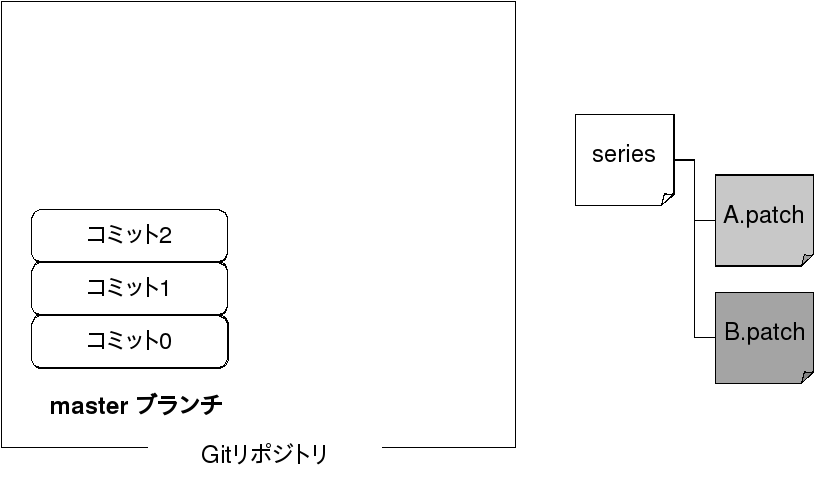
\includegraphics[width=0.8\hsize]{image201509/gbp-pq0_mono.png}
\end{center}


\subsection{gbp pq import}

  \begin{enumerate}
   \item HEAD をpatch-queue/master ブランチとしてチェックアウト
   \item debian/patches/series にあるパッチをコミット
  \end{enumerate}

\begin{center}
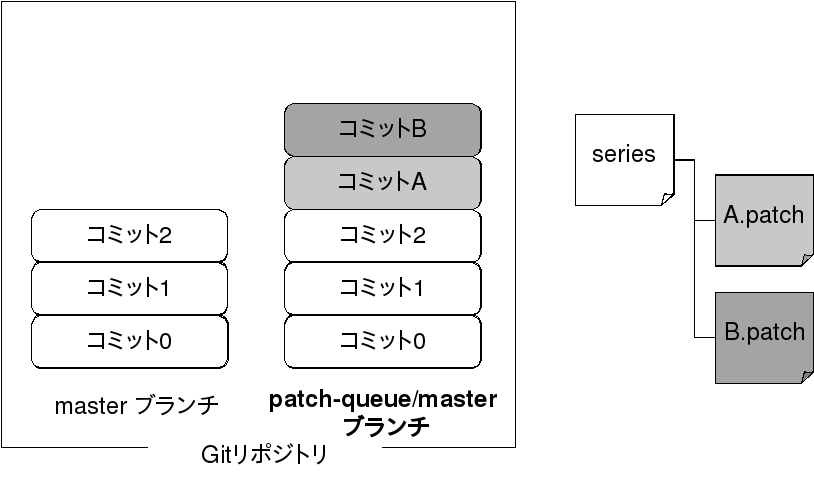
\includegraphics[width=0.8\hsize]{image201509/gbp-pq1_mono.png}
\end{center}


\subsection{修正 \& git commit}

  \begin{enumerate}
   \item Upstream ソースコードの修正
   \item git commit
  \end{enumerate}

\begin{center}
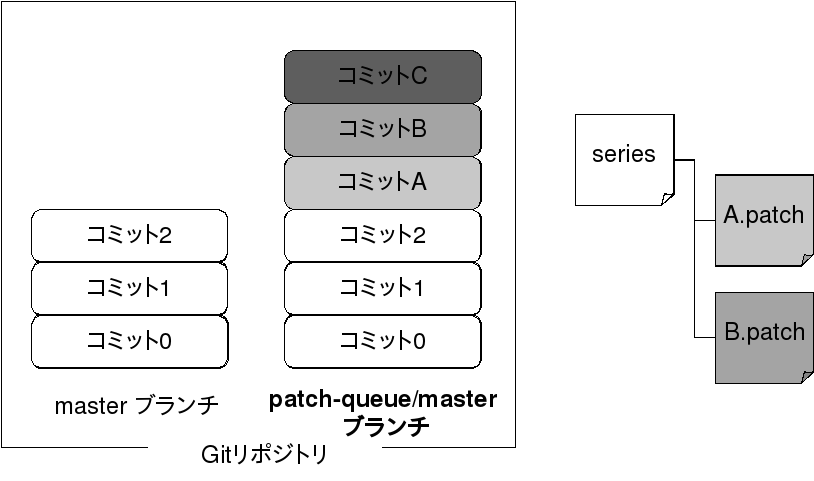
\includegraphics[width=0.8\hsize]{image201509/gbp-pq2_mono.png}
\end{center}


\subsection{gbp pq export}
  \begin{enumerate}
   \item patch-queue/master と master ブランチの差分をパッチとして debian/patches に出力
   \item debian/patches/series を更新
   \item master ブランチをチェックアウト
  \end{enumerate}

\begin{center}
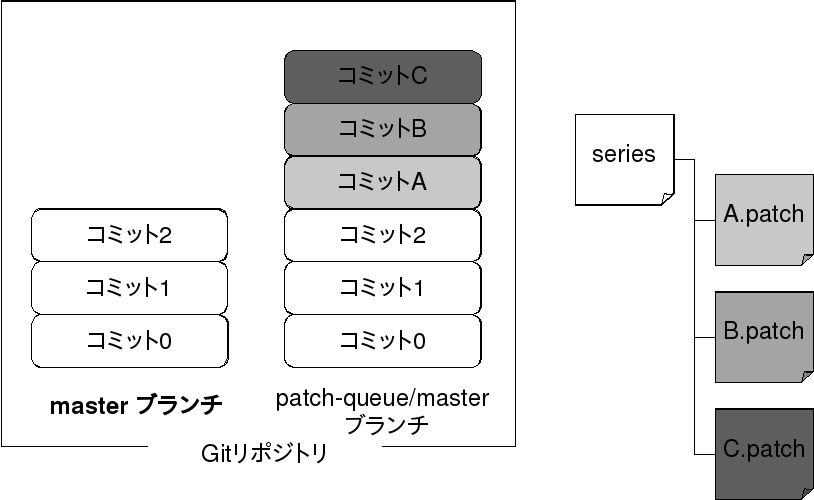
\includegraphics[width=0.8\hsize]{image201509/gbp-pq3_mono.png}
\end{center}
  
  

\subsection{git commit}
  \begin{enumerate}
   \item パッチ更新をリポジトリにコミット
  \end{enumerate}

\begin{center}
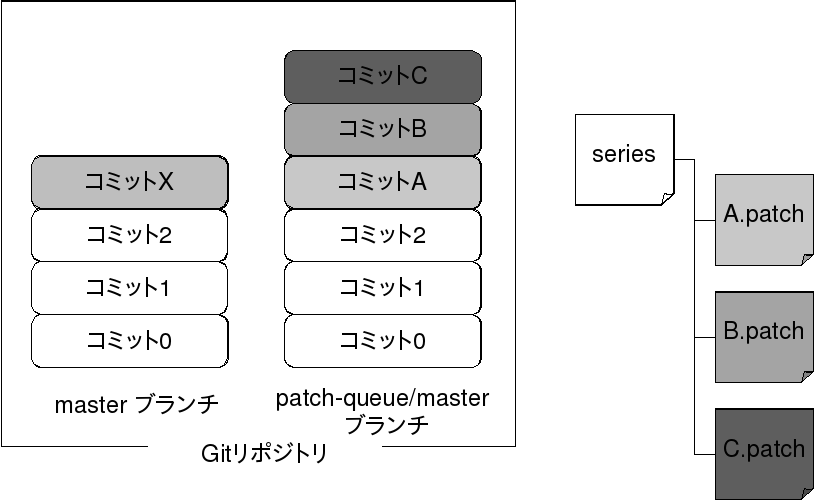
\includegraphics[width=0.8\hsize]{image201509/gbp-pq4_mono.png}
\end{center}

\subsection{まとめ}

\begin{itemize}
\item gbp (git buildpackage)はデファクトスタンダート
\item gbp import-* でリポジトリ取り込み
  
  \texttt{--pristine-tar} を忘れずに
\item gbp dch で debian/changelog を更新
\item gbp buildpackage でパッケージビルド
\item gbp pq でパッチ操作
\end{itemize}

%-------------------------------------------------------------------------------
\dancersection{Debian Trivia Quiz}{}
%-------------------------------------------------------------------------------

ところで、みなさん Debian 関連の話題においついていますか?Debian関連の話
題はメーリングリストをよんでいると追跡できます。ただよんでいるだけではは
りあいがないので、理解度のテストをします。特に一人だけでは意味がわからな
いところもあるかも知れません。みんなで一緒に読んでみましょう。

今回の出題範囲は\url{debian-devel-announce@lists.debian.org} や \url{debian-devel@lists.debian.org}に投稿された
内容とDebian Project Newsからです。

\begin{multicols}{2}
%; whizzy-master ../debianmeetingresume201311.tex
% $B0J>e$N@_Dj$r$7$F$$$k$?$a!"$3$N%U%!%$%k$G(B M-x whizzytex $B$9$k$H!"(Bwhizzytex$B$,MxMQ$G$-$^$9!#(B
%

\santaku
{Debian 8.1 $B$,%j%j!<%9$5$l$^$7$?!#$$$D$@$C$?$G$7$g$&$+!)(B}
{2015/6/6}
{2015/6/13}
{2015/6/20}
{A}
{$B$$$/$D$+$N@H<e@-BP:v$d!"%P%0%U%#%C%/%9$,9T$o$l$?%Q%C%1!<%8$,<h$j9~$^$l$^$7$?!#(BDebian 8(Jessie)$B$r%$%s%9%H!<%k$7$?$P$+$j$N?M$O!"AaB.%"%C%W%0%l!<%I$7$^$7$g$&!*(B}

\santaku
{2015/6/10$B$K$F!"(Bunstable$BHG$N%=!<%9%Q%C%1!<%8$N?t$O$$$/$D$K$J$C$?$G$7$g$&$+!)(B}
{21,000}
{22,000}
{23,000}
{B}
{$B?k$K(B22,000$B$rD6$($?$=$&$G$9!#%P%$%J%j%Q%C%1!<%8$N?t$O(B45,542$B$H$N;v!#1W!9A}$($F$$$/$h$&$G$9!#(B}

\santaku
{AutomaticDebugPackages$B$NDs0F$H$O2?!)(B}
{$BBgE}0l(BDebian$B$N4d>>$5$s$N%G%P%C%0%Q%C%1!<%8$N7o$r<B;\$9$k(B}
{$B<+F0$G%G%P%C%0=PMh$k$h$&$K$9$k(B}
{-dbg$B%Q%C%1!<%8$r;_$a!"(B.ddeb$B%Q%C%1!<%8$r:n$k(B}
{C}
{$B:#$^$G!"%G%P%C%0%7%s%\%k$O(B-dbg$B%Q%C%1!<%8$GG[I[$5$l$F$$$^$7$?!#$7$+$7$J$,$i!"$3$A$i$N(B-dbg$B%Q%C%1!<%8$OB>$N%G%P%C%0$H$O2?$i4X78$N$J$$%Q%C%1!<%8$H0l=o$K(Bmirror$B$5$l$k$?$a!"(B-dbg$B%Q%C%1!<%8$NMxMQ<T$,$H$F$b>/$J$$$K$b$+$+$o$i$:!"(Bmirror$B@h$N;q8;$r$=$NJ,>CHq$7$F$7$^$$$^$9!#:#2s$NDs0F$O!"%G%P%C%0%7%s%\%k(B.ddeb$B$H$$$&%Q%C%1!<%8$K$7$F$7$^$$!"$3$A$i$N%Q%C%1!<%8$K$D$$$F$O(Bmirror$B@h$b8:$i$9!J$7$J$$!)!K$H$$$&;v$r8!F$$9$k$b$N$G$9!#(B}





%; whizzy-master ../debianmeetingresume201311.tex
% $B0J>e$N@_Dj$r$7$F$$$k$?$a!"$3$N%U%!%$%k$G(B M-x whizzytex $B$9$k$H!"(Bwhizzytex$B$,MxMQ$G$-$^$9!#(B
%

\santaku
{6/22$B$K$F!"(Bbackport$B$N%A!<%`$,!"FCDj$N>r7o$rK~$?$9%Q%C%1!<%8$r$4$C$=$j>C$7$?$N$O!"$I$N(Bbackports?}
{squeeze-backports}
{wheezy-backports}
{jessie-backports}
{B}
{jessie$B$GMxMQ$G$-$J$$%Q%C%1!<%8$r!"(Bwheezy-backports$B$+$i$4$C$=$j>C$7$?$H$N$3$H$G$9!#(Bbackports$B$K4^$^$l$k$I$N%Q%C%1!<%8$,$I$&$J$C$F$$$k$+!)$I$&$7$FM_$7$$$+!)$K$D$$$F$O!"(Bfreeze$B$N4|4V$H(Bfreeze$B8e$N$o$:$+$J4|4V$N4V$K!"(Bbackport$BC4Ev$+$i(Bbackports$B%A!<%`$K<+H/E*$K%?%$%`%j!<$KAjCL$7$FMh$FM_$7$$$H$N4+9p$b9T$o$l$^$7$?!#(B}

\santaku
{7/7$B$K$F!"(Bsid$B$G$O!"FCDj%P!<%8%g%s$N(BGCC$B$H(Blibstdc++$B$G%3%s%Q%$%k!&F0:n=PMh$k$h$&$K$7$FM_$7$$;]$N%"%J%&%s%9$,N.$l$^$7$?!#$I$NAH$_9g$o$;!)(B}
{gcc 6/libstdc++6}
{gcc 4/libstdc++5}
{gcc 5/libstdc++6}
{C}
{$B$^$:$O!"(BDebian sid$B$G$O!"(Bgcc 5/libstdc++6$B$G%3%s%Q%$%k!&F0:n=PMh$k$h$&$K%Q%C%1!<%8%a%s%F%J$NJ}$O=$@5BP1~$r$7$FM_$7$$;]$N%"%J%&%s%9$,$"$j$^$7$?!#:#2s!"(BABI$B%Y!<%9$G$bJQ99$K$J$C$?$j!"(BC++11$B$KBP1~$H$J$C$?$j$G1F6A$,=t!9H/@8$7$^$9!#$^$?!"$3$N1F6A$G!"(BGFortran$BB&$b(Bmodule 14$B$X0\9T$H$J$k$N$G!"(BGFortran$B$r;H$C$F$$$k%Q%C%1!<%8%a%s%F%J$bBP1~$,I,MW$H$N$3$H$G$9!#(B}

\santaku
{7/8$B$K$F!"J#?t$N(Bupstream$B$+$iDs6!$5$l$F$$$k(Blibav*$B72$N%i%$%V%i%j$K$D$$$F!"Ds6!85$N(Bupstream$B$rJQ99$9$k$H$NO"Mm$,$"$j$^$7$?!#$I$N(Bupstream$B$KJQ99$H$J$C$?$N$G$7$g$&$+!)(B}
{FFmpeg}
{libav.org}
{VideoLAN}
{A}
{libav*$B$H$$$&%^%k%A%a%G%#%"$N%G!<%?$r07$&%i%$%V%i%j$J$N$G$9$,!"0lC6(Blibav.org$B$,Ds6!$7$F$$$k$b$N$KJQ99$H$J$C$?$N$G$9$,!"$^$?(BFFmpeg$B$,Ds6!$7$F$$$k$b$N$KLa$C$F$-$?>u67$G$9!#5DO@$N%5%^%j$O(B https://wiki.debian.org/Debate/libav-provider/ffmpeg}

\santaku
{DPL$B$N(BNeil MacGovern$B$,(Breddit$B$K3+$$$?!V(BDPL$B$@$1$I!"2?$+<ALd$"$k!)!W$H$$$&%9%l$G!"(BDPL$B$K$H$C$F$b@($$$H;W$&%G%#%9%H%j%S%e!<%7%g%s$H$7$F$"$2$i$l$F$?$b$N$O$I$l!)(B}
{$BEvA3(BDebian$B$C$7$g!*(B}
{ArchLinux}
{ubuntu}
{B}
{$B%9%l$N=;?M$N<ALd$K!"(BDPL$B$,(BArchLinux$B$,@($$$HEz$($F$$$^$7$?!#(Bwiki$B$N=<<B$V$j$,$H$K$+$/AG@2$i$7$$$H$N$3$H!#(B}

\santaku
{7/20$B$K(Bdgit$B$N?7$7$$%P!<%8%g%s$N$b$N$,%j%j!<%9$5$l$^$7$?!#$I$N%P!<%8%g%s$K$J$C$?!)(B}
{0.1}
{0.3}
{1.0}
{C}
{Debian$B%"!<%+%$%V$r(Bgit$B$GA`:n$G$-$k%D!<%k$N(Bdgit$B$,(B1.0$B$,%j%j!<%9$5$l$?$H$N$3$H$G$9!#AaB.(Bdebian sid$B$K<}O?$5$l$F$$$^$9!#(Bdgit clone package$BL>$H$9$k$H!"(Bhttps://git.dgit.debian.org/ $B$G4IM}$5$l$F$$$k$b$N$,<j85$K(Bclone$B$5$l$^$9!#(B}

\santaku
{7/21$B$K(B Debian Installer Stretch Alpha 1$B$,%j%j!<%9$5$l$^$7$?!#JQ99E@$O0J2<$N$I$l!)(B}
{UEFI$B%V!<%H$rEk:\(B}
{$B%M%C%H%o!<%/(BIF$B$,(BMAC$B%"%I%l%9$K$J$k(B}
{$B%$%s%9%H!<%k;~$N(BUI$B$,(Btext$B%b!<%I$+$i(Bgraphical$B%b!<%I$K$J$C$?(B}
{C}
{Strech$B$GMxMQ$5$l$k$G$"$m$&!"%$%s%9%H!<%i%W%m%0%i%`$N&A(B1$B$,%j%j!<%9$5$l$^$7$?!#$b$A$m$s!"(BStrech$B$,%j%j!<%9$5$l$?$o$1$G$O$J$$$N$GCm0U!#JQ99E@$O?t!9$"$j!"%G%U%)%k%H$N(BCPU$B%"!<%-%F%/%A%c$,(Bamd64$B$K$J$C$?$j$7$?!#>\$7$/$O(Bdebian-devel-announce$B$r;2>H(B}

%; whizzy-master ../debianmeetingresume201311.tex
% $B0J>e$N@_Dj$r$7$F$$$k$?$a!"$3$N%U%!%$%k$G(B M-x whizzytex $B$9$k$H!"(Bwhizzytex$B$,MxMQ$G$-$^$9!#(B
%

\santaku
{2015/10/22$B$N(BDPN$B$N%a!<%k$+$iDj4|E*$K$J$,$l$F$$$?$$$/$D$+$N%H%T%C%/$,(BWeb$B$N$_$K7G<($5$l$k$h$&$K$J$j$^$7$?!#$I$3$K7G<($5$l$k!)(B}
{http://www.debian.or.jp/}
{http://www.debian.org/}
{http://bits.debian.org/}
{C}
{2015/10/22$B$N(BDPN$B$N%a!<%k$+$i!"=>MhN.$l$F$$$?(BDPN$B$N%a!<%k$N9=@.$,:~?7$5$l$^$7$?!#$3$A$i$KH<$$!"%;%-%e%j%F%#$K$D$$$F$N%"%J%&%s%9$H!"?7$7$$(BDD/DM$B$N%"%J%&%s%9$O!"(BDPN$B$N%a!<%k$K$O4^$^$l$:!"(BWeb$B%Z!<%8$K7G:\$5$l$k$N$_$H$J$j$^$7$?!#(B}

\santaku
{2015/11/7$B$K$F!"$H$"$k%$%s%9%?%s%H%a%C%;%s%8%c!<MQ%W%m%H%3%k$N%5!<%S%9$,A4(BDebian Developer$B$G;H$($k$h$&$K$J$C$?$H$N%"%J%&%s%9$,$"$j$^$7$?!#%W%m%H%3%k$NL>A0$O<!$N$I$l!)(B}
{XMPP}
{IRC}
{IP Messanger}
{A}
{XMPP$B$O%*!<%W%s$J%$%s%9%?%s%H%a%C%;%s%8%c!<MQ%W%m%H%3%k$N#1$D!#$J$*!"(BDebian$B4X78<T$NMxMQ$K$"$?$C$F>\$7$/$O!"(Bhttp://rtc.debian.org$B$r;2>H!#(B}

\santaku
{2015/10/30$B$K$F!"(BDebian$B$K$F!"(B2$B2sL\$N8xJg$,9T$o$l$?Lr$^$o$j$O<!$N$I$l!)(B}
{2016 DPN}
{technical commitee}
{2016 Debian JP$B2qD9(B}
{B}
{2$BL>$[$I!"(BDebian Developer$B$NJ}$G(Btechnical comittee$B$G3hLv$G$-$kJ}Jg=8$H$N$3$H$G$9!#8=?&(Btechnical comittee$B$N?M$i$,!"(B2015/12/31$B$GG$4|$,@Z$l$F$7$^$&$H$$$&$3$H$G!"$=$l$^$G$K8uJd<T$r5s$2$kI,MW$,$"$k$H$N$3$H$G$9!#(B}



\end{multicols}

%for less page
%\printindex

\newpage

\begin{center}
本資料のライセンスについて
\end{center}

本資料はフリー・ソフトウェアです。あなたは、Free Software
Foundation が公表したGNU GENERAL PUBLIC LICENSEの「バージョン2」もしくはそれ以降
が定める条項に従って本プログラムを再頒布または変更することができ
ます。

本プログラムは有用とは思いますが、頒布にあたっては、市場性及び特
定目的適合性についての暗黙の保証を含めて、いかなる保証も行ないま
せん。詳細についてはGNU GENERAL PUBLIC LICENSE をお読みください。

\begin{multicols}{2}
 \begin{fontsize}{6}{6}
 \begin{verbatim}
		    GNU GENERAL PUBLIC LICENSE
		       Version 2, June 1991

 Copyright (C) 1989, 1991 Free Software Foundation, Inc.
	51 Franklin St, Fifth Floor, Boston, MA  02110-1301  USA
 Everyone is permitted to copy and distribute verbatim copies
 of this license document, but changing it is not allowed.

			    Preamble

  The licenses for most software are designed to take away your
freedom to share and change it.  By contrast, the GNU General Public
License is intended to guarantee your freedom to share and change free
software--to make sure the software is free for all its users.  This
General Public License applies to most of the Free Software
Foundation's software and to any other program whose authors commit to
using it.  (Some other Free Software Foundation software is covered by
the GNU Library General Public License instead.)  You can apply it to
your programs, too.

  When we speak of free software, we are referring to freedom, not
price.  Our General Public Licenses are designed to make sure that you
have the freedom to distribute copies of free software (and charge for
this service if you wish), that you receive source code or can get it
if you want it, that you can change the software or use pieces of it
in new free programs; and that you know you can do these things.

  To protect your rights, we need to make restrictions that forbid
anyone to deny you these rights or to ask you to surrender the rights.
These restrictions translate to certain responsibilities for you if you
distribute copies of the software, or if you modify it.

  For example, if you distribute copies of such a program, whether
gratis or for a fee, you must give the recipients all the rights that
you have.  You must make sure that they, too, receive or can get the
source code.  And you must show them these terms so they know their
rights.

  We protect your rights with two steps: (1) copyright the software, and
(2) offer you this license which gives you legal permission to copy,
distribute and/or modify the software.

  Also, for each author's protection and ours, we want to make certain
that everyone understands that there is no warranty for this free
software.  If the software is modified by someone else and passed on, we
want its recipients to know that what they have is not the original, so
that any problems introduced by others will not reflect on the original
authors' reputations.

  Finally, any free program is threatened constantly by software
patents.  We wish to avoid the danger that redistributors of a free
program will individually obtain patent licenses, in effect making the
program proprietary.  To prevent this, we have made it clear that any
patent must be licensed for everyone's free use or not licensed at all.

  The precise terms and conditions for copying, distribution and
modification follow.

		    GNU GENERAL PUBLIC LICENSE
   TERMS AND CONDITIONS FOR COPYING, DISTRIBUTION AND MODIFICATION

  0. This License applies to any program or other work which contains
a notice placed by the copyright holder saying it may be distributed
under the terms of this General Public License.  The "Program", below,
refers to any such program or work, and a "work based on the Program"
means either the Program or any derivative work under copyright law:
that is to say, a work containing the Program or a portion of it,
either verbatim or with modifications and/or translated into another
language.  (Hereinafter, translation is included without limitation in
the term "modification".)  Each licensee is addressed as "you".

Activities other than copying, distribution and modification are not
covered by this License; they are outside its scope.  The act of
running the Program is not restricted, and the output from the Program
is covered only if its contents constitute a work based on the
Program (independent of having been made by running the Program).
Whether that is true depends on what the Program does.

  1. You may copy and distribute verbatim copies of the Program's
source code as you receive it, in any medium, provided that you
conspicuously and appropriately publish on each copy an appropriate
copyright notice and disclaimer of warranty; keep intact all the
notices that refer to this License and to the absence of any warranty;
and give any other recipients of the Program a copy of this License
along with the Program.

You may charge a fee for the physical act of transferring a copy, and
you may at your option offer warranty protection in exchange for a fee.

  2. You may modify your copy or copies of the Program or any portion
of it, thus forming a work based on the Program, and copy and
distribute such modifications or work under the terms of Section 1
above, provided that you also meet all of these conditions:

    a) You must cause the modified files to carry prominent notices
    stating that you changed the files and the date of any change.

    b) You must cause any work that you distribute or publish, that in
    whole or in part contains or is derived from the Program or any
    part thereof, to be licensed as a whole at no charge to all third
    parties under the terms of this License.

    c) If the modified program normally reads commands interactively
    when run, you must cause it, when started running for such
    interactive use in the most ordinary way, to print or display an
    announcement including an appropriate copyright notice and a
    notice that there is no warranty (or else, saying that you provide
    a warranty) and that users may redistribute the program under
    these conditions, and telling the user how to view a copy of this
    License.  (Exception: if the Program itself is interactive but
    does not normally print such an announcement, your work based on
    the Program is not required to print an announcement.)

These requirements apply to the modified work as a whole.  If
identifiable sections of that work are not derived from the Program,
and can be reasonably considered independent and separate works in
themselves, then this License, and its terms, do not apply to those
sections when you distribute them as separate works.  But when you
distribute the same sections as part of a whole which is a work based
on the Program, the distribution of the whole must be on the terms of
this License, whose permissions for other licensees extend to the
entire whole, and thus to each and every part regardless of who wrote it.

Thus, it is not the intent of this section to claim rights or contest
your rights to work written entirely by you; rather, the intent is to
exercise the right to control the distribution of derivative or
collective works based on the Program.

In addition, mere aggregation of another work not based on the Program
with the Program (or with a work based on the Program) on a volume of
a storage or distribution medium does not bring the other work under
the scope of this License.

  3. You may copy and distribute the Program (or a work based on it,
under Section 2) in object code or executable form under the terms of
Sections 1 and 2 above provided that you also do one of the following:

    a) Accompany it with the complete corresponding machine-readable
    source code, which must be distributed under the terms of Sections
    1 and 2 above on a medium customarily used for software interchange; or,

    b) Accompany it with a written offer, valid for at least three
    years, to give any third party, for a charge no more than your
    cost of physically performing source distribution, a complete
    machine-readable copy of the corresponding source code, to be
    distributed under the terms of Sections 1 and 2 above on a medium
    customarily used for software interchange; or,

    c) Accompany it with the information you received as to the offer
    to distribute corresponding source code.  (This alternative is
    allowed only for noncommercial distribution and only if you
    received the program in object code or executable form with such
    an offer, in accord with Subsection b above.)

The source code for a work means the preferred form of the work for
making modifications to it.  For an executable work, complete source
code means all the source code for all modules it contains, plus any
associated interface definition files, plus the scripts used to
control compilation and installation of the executable.  However, as a
special exception, the source code distributed need not include
anything that is normally distributed (in either source or binary
form) with the major components (compiler, kernel, and so on) of the
operating system on which the executable runs, unless that component
itself accompanies the executable.

If distribution of executable or object code is made by offering
access to copy from a designated place, then offering equivalent
access to copy the source code from the same place counts as
distribution of the source code, even though third parties are not
compelled to copy the source along with the object code.

  4. You may not copy, modify, sublicense, or distribute the Program
except as expressly provided under this License.  Any attempt
otherwise to copy, modify, sublicense or distribute the Program is
void, and will automatically terminate your rights under this License.
However, parties who have received copies, or rights, from you under
this License will not have their licenses terminated so long as such
parties remain in full compliance.

  5. You are not required to accept this License, since you have not
signed it.  However, nothing else grants you permission to modify or
distribute the Program or its derivative works.  These actions are
prohibited by law if you do not accept this License.  Therefore, by
modifying or distributing the Program (or any work based on the
Program), you indicate your acceptance of this License to do so, and
all its terms and conditions for copying, distributing or modifying
the Program or works based on it.

  6. Each time you redistribute the Program (or any work based on the
Program), the recipient automatically receives a license from the
original licensor to copy, distribute or modify the Program subject to
these terms and conditions.  You may not impose any further
restrictions on the recipients' exercise of the rights granted herein.
You are not responsible for enforcing compliance by third parties to
this License.

  7. If, as a consequence of a court judgment or allegation of patent
infringement or for any other reason (not limited to patent issues),
conditions are imposed on you (whether by court order, agreement or
otherwise) that contradict the conditions of this License, they do not
excuse you from the conditions of this License.  If you cannot
distribute so as to satisfy simultaneously your obligations under this
License and any other pertinent obligations, then as a consequence you
may not distribute the Program at all.  For example, if a patent
license would not permit royalty-free redistribution of the Program by
all those who receive copies directly or indirectly through you, then
the only way you could satisfy both it and this License would be to
refrain entirely from distribution of the Program.

If any portion of this section is held invalid or unenforceable under
any particular circumstance, the balance of the section is intended to
apply and the section as a whole is intended to apply in other
circumstances.

It is not the purpose of this section to induce you to infringe any
patents or other property right claims or to contest validity of any
such claims; this section has the sole purpose of protecting the
integrity of the free software distribution system, which is
implemented by public license practices.  Many people have made
generous contributions to the wide range of software distributed
through that system in reliance on consistent application of that
system; it is up to the author/donor to decide if he or she is willing
to distribute software through any other system and a licensee cannot
impose that choice.

This section is intended to make thoroughly clear what is believed to
be a consequence of the rest of this License.

  8. If the distribution and/or use of the Program is restricted in
certain countries either by patents or by copyrighted interfaces, the
original copyright holder who places the Program under this License
may add an explicit geographical distribution limitation excluding
those countries, so that distribution is permitted only in or among
countries not thus excluded.  In such case, this License incorporates
the limitation as if written in the body of this License.

  9. The Free Software Foundation may publish revised and/or new versions
of the General Public License from time to time.  Such new versions will
be similar in spirit to the present version, but may differ in detail to
address new problems or concerns.

Each version is given a distinguishing version number.  If the Program
specifies a version number of this License which applies to it and "any
later version", you have the option of following the terms and conditions
either of that version or of any later version published by the Free
Software Foundation.  If the Program does not specify a version number of
this License, you may choose any version ever published by the Free Software
Foundation.

  10. If you wish to incorporate parts of the Program into other free
programs whose distribution conditions are different, write to the author
to ask for permission.  For software which is copyrighted by the Free
Software Foundation, write to the Free Software Foundation; we sometimes
make exceptions for this.  Our decision will be guided by the two goals
of preserving the free status of all derivatives of our free software and
of promoting the sharing and reuse of software generally.

			    NO WARRANTY

  11. BECAUSE THE PROGRAM IS LICENSED FREE OF CHARGE, THERE IS NO WARRANTY
FOR THE PROGRAM, TO THE EXTENT PERMITTED BY APPLICABLE LAW.  EXCEPT WHEN
OTHERWISE STATED IN WRITING THE COPYRIGHT HOLDERS AND/OR OTHER PARTIES
PROVIDE THE PROGRAM "AS IS" WITHOUT WARRANTY OF ANY KIND, EITHER EXPRESSED
OR IMPLIED, INCLUDING, BUT NOT LIMITED TO, THE IMPLIED WARRANTIES OF
MERCHANTABILITY AND FITNESS FOR A PARTICULAR PURPOSE.  THE ENTIRE RISK AS
TO THE QUALITY AND PERFORMANCE OF THE PROGRAM IS WITH YOU.  SHOULD THE
PROGRAM PROVE DEFECTIVE, YOU ASSUME THE COST OF ALL NECESSARY SERVICING,
REPAIR OR CORRECTION.

  12. IN NO EVENT UNLESS REQUIRED BY APPLICABLE LAW OR AGREED TO IN WRITING
WILL ANY COPYRIGHT HOLDER, OR ANY OTHER PARTY WHO MAY MODIFY AND/OR
REDISTRIBUTE THE PROGRAM AS PERMITTED ABOVE, BE LIABLE TO YOU FOR DAMAGES,
INCLUDING ANY GENERAL, SPECIAL, INCIDENTAL OR CONSEQUENTIAL DAMAGES ARISING
OUT OF THE USE OR INABILITY TO USE THE PROGRAM (INCLUDING BUT NOT LIMITED
TO LOSS OF DATA OR DATA BEING RENDERED INACCURATE OR LOSSES SUSTAINED BY
YOU OR THIRD PARTIES OR A FAILURE OF THE PROGRAM TO OPERATE WITH ANY OTHER
PROGRAMS), EVEN IF SUCH HOLDER OR OTHER PARTY HAS BEEN ADVISED OF THE
POSSIBILITY OF SUCH DAMAGES.

		     END OF TERMS AND CONDITIONS

	    How to Apply These Terms to Your New Programs

  If you develop a new program, and you want it to be of the greatest
possible use to the public, the best way to achieve this is to make it
free software which everyone can redistribute and change under these terms.

  To do so, attach the following notices to the program.  It is safest
to attach them to the start of each source file to most effectively
convey the exclusion of warranty; and each file should have at least
the "copyright" line and a pointer to where the full notice is found.

    <one line to give the program's name and a brief idea of what it does.>
    Copyright (C) <year>  <name of author>

    This program is free software; you can redistribute it and/or modify
    it under the terms of the GNU General Public License as published by
    the Free Software Foundation; either version 2 of the License, or
    (at your option) any later version.

    This program is distributed in the hope that it will be useful,
    but WITHOUT ANY WARRANTY; without even the implied warranty of
    MERCHANTABILITY or FITNESS FOR A PARTICULAR PURPOSE.  See the
    GNU General Public License for more details.

    You should have received a copy of the GNU General Public License
    along with this program; if not, write to the Free Software
    Foundation, Inc., 51 Franklin St, Fifth Floor, Boston, MA  02110-1301 USA


Also add information on how to contact you by electronic and paper mail.

If the program is interactive, make it output a short notice like this
when it starts in an interactive mode:

    Gnomovision version 69, Copyright (C) year  name of author
    Gnomovision comes with ABSOLUTELY NO WARRANTY; for details type `show w'.
    This is free software, and you are welcome to redistribute it
    under certain conditions; type `show c' for details.

The hypothetical commands `show w' and `show c' should show the appropriate
parts of the General Public License.  Of course, the commands you use may
be called something other than `show w' and `show c'; they could even be
mouse-clicks or menu items--whatever suits your program.

You should also get your employer (if you work as a programmer) or your
school, if any, to sign a "copyright disclaimer" for the program, if
necessary.  Here is a sample; alter the names:

  Yoyodyne, Inc., hereby disclaims all copyright interest in the program
  `Gnomovision' (which makes passes at compilers) written by James Hacker.

  <signature of Ty Coon>, 1 April 1989
  Ty Coon, President of Vice

This General Public License does not permit incorporating your program into
proprietary programs.  If your program is a subroutine library, you may
consider it more useful to permit linking proprietary applications with the
library.  If this is what you want to do, use the GNU Library General
Public License instead of this License.
 \end{verbatim}
 \end{fontsize}
\end{multicols}

\begin{center}
ソースコードについて
\end{center}

ソースコードは Git を使って\url{git://anonscm.debian.org/tokyodebian/monthly-report.git}
からダウンロードできます。以下に方法を示します。

\begin{commandline}
$ git clone git://anonscm.debian.org/tokyodebian/monthly-report.git
\end{commandline}
%$

% 問題と回答が同じみひらきにならないようにする->GPLページを挟んだので問題なし
\newpage
%-------------------------------------------------------------------------------
\dancersection{Debian Trivia Quiz 問題回答}{}
%-------------------------------------------------------------------------------

 Debian Trivia Quiz の問題回答です。
 あなたは何問わかりましたか? \\
 %回答はdebianmeetingresume2014-fuyu.jqzというファイルに生成されるので、
 %それを手動でコピペして使う。
 % ここからコピペ
 % FIXME 問題が全部はいったらコピペすること
 %(progn (next-line 1)(insert-file "debianmeetingresume2013-fuyu.jqz") )
1. A いくつかの脆弱性対策や、バグフィックスが行われたパッケージが取り込まれました。Debian 8(Jessie)をインストールしたばかりの人は、早速アップグレードしましょう!\\
2. B 遂に22,000を超えたそうです。バイナリパッケージの数は45,542との事。益々増えていくようです。\\
3. C 今まで、デバッグシンボルは-dbgパッケージで配布されていました。こちらの-dbgパッケージは他のデバッグとは何ら関係のないパッケージと一緒にmirrorされ、利用者がとても少ないが、mirror先の資源を消費します。提案は、デバッグシンボル.ddebというパッケージにし、mirror先も減らす(しない?)という事を検討するものです。\\
4. B jessieで利用できないパッケージを、wheezy-backportsからごっそり消したとのことです。backportsに含まれるどのパッケージがどうなっているか?どうして欲しいか?については、freezeの期間とfreeze後のわずかな期間の間に、backport担当からbackportsチームに自発的にタイムリーに相談して来て欲しいとの勧告も行われました。\\
5. C まずは、Debian sidでは、gcc 5/libstdc++6でコンパイル・動作出来るようにパッケージメンテナの方は修正対応をして欲しい旨のアナウンスがありました。今回、ABIベースでも変更になったり、C++11に対応となったりで影響が諸々発生します。また、この影響で、GFortran側もmodule 14へ移行となるので、GFortranを使っているパッケージメンテナも対応が必要とのことです。\\
6. A libav*というマルチメディアのデータを扱うライブラリなのですが、一旦libav.orgが提供しているものに変更となったのですが、またFFmpegが提供しているものに戻ってきた状況です。議論のサマリは https://wiki.debian.org/Debate/libav-provider/ffmpeg\\
7. B 質問に、DPLがArchLinuxが凄いと答えていました。wikiの充実ぶりがとにかく素晴らしいとのこと。\\
8. C Debianアーカイブをgitで操作できるツールのdgitが1.0がリリースされたとのことです。早速debian sidに収録されています。dgit clone package名とすると、https://git.dgit.debian.org/ で管理されているものが手元にcloneされます。\\
9. C Strechで利用されるであろう、インストーラプログラムのα1がリリースされました。もちろん、Strechがリリースされたわけではないので注意。変更点は数々あり、デフォルトのCPUアーキテクチャがamd64になったりした。詳しくはdebian-devel-announceを参照\\
10. C 2015/10/22のDPNのメールから、従来流れていたDPNのメールの構成が刷新されました。こちらに伴い、セキュリティについてのアナウンスと、新しいDD/DMのアナウンスは、DPNのメールには含まれず、Webページに掲載されるのみとなりました。\\
11. A XMPPはオープンなインスタントメッセンジャー用プロトコルの1つ。なお、Debian関係者の利用にあたって詳しくは、http://rtc.debian.orgを参照。\\
12. B 2名、Debian Developerの方でtechnical comitteeで活躍できる方募集とのことです。現職technical comitteeの人らが、2015/12/31で任期が切れてしまうため、それまでに候補者を挙げる必要があるとのこと。

% add page to even number
%\newpage
%\cleartoevenpage

\newpage
\thispagestyle{empty}\mbox{}
\newpage

\thispagestyle{empty}
{
\large
\begin{itembox}{\bf 『あんどきゅめんてっど でびあん』について}
本書は、東京および関西周辺で毎月行なわれている『東京エリア Debian 勉強会』および
『関西 Debian 勉強会』で
使用された資料・小ネタ・必殺技などを一冊にまとめたものです。
% FIXME: 範囲を修正すること。
収録範囲は2015/06〜2015/11まで
東京エリアは第127回から第133回までおよび、
関西エリアは第99回から第104回まで(関西第99-101回,104回はもくもく会、LTのため収録無し)。
内容は無保証、つっこみなどがあれば勉強会にて。
\end{itembox}
}

\vspace*{13cm}
{\color{dancerlightblue}\rule{\hsize}{1mm}}
\vspace{2mm}

\includegraphics[width=2cm]{image200502/openlogo-nd.eps}
\noindent \Large \bf あんどきゅめんてっど でびあん 2015年冬号\\
\noindent \normalfont 2015年12月31日 \hspace{5mm}  初版第1刷発行\\
\noindent \normalfont 東京エリア Debian 勉強会/関西Debian 勉強会 (編集・印刷・発行)\\
{\color{dancerdarkblue}\rule{\hsize}{1mm}}

\end{document}
